%c.f. (also contains references to docs) https://git.ias.informatik.tu-darmstadt.de/thesis/beamer/-/blob/8c27d60b328220db8a4f64275d6f94a300b48cdc/texmf/doc/latex/tuda-ci/example/DEMO-TUDaBeamer.tex

\documentclass[
	ngerman,%globale Übergabe der Hauptsprache
	aspectratio=169,%Beamer eigene Option zum Umschalten des Formates
	color={accentcolor=8c},
	logo=true,%Logo auf Folgeseiten
	colorframetitle=true,%Akzentfarbe auch im Frametitle
    %logofile=example-image, %Falls die Logo Dateien nicht vorliegen
    authorontitle=true,
	]{tudabeamer}
\usepackage[main=english]{babel}

\usepackage{tikz}
\usetikzlibrary{3d, angles, animations, arrows, arrows.meta, arrows.spaced, automata, babel, backgrounds, bending, calc, calendar, chains, circuits.ee.IEC, circuits.logic.CDH, circuits.logic.IEC, circuits.logic.US, datavisualization, datavisualization.formats.functions, datavisualization.polar, decorations, decorations.footprints, decorations.fractals, decorations.markings, decorations.pathmorphing, decorations.pathreplacing, decorations.shapes, decorations.text, er, external, fadings, fit, fixedpointarithmetic, folding, fpu, graphs, graphs.standard, intersections, lindenmayersystems, math, matrix, patterns, patterns.meta, perspective, petri, plotmarks, positioning, quotes, rdf, scopes, shadings, shadows, shadows.blur, shapes, shapes.arrows, shapes.callouts, shapes.gates.logic.IEC, shapes.gates.logic.US, shapes.geometric, shapes.misc, shapes.multipart, shapes.symbols, spy, svg.path, through, tikzmark, topaths, trees, turtle, views}
\tikzset{
     %set default line width to 0.75pt
    every picture/.style={line width=0.75pt},
    data-box/.style={
        draw,
        minimum width=1.5em,
        minimum height=1.5em,
    },
    hist-box/.style={
        draw,
        minimum width=3em,
        minimum height=3em,
    },
    send-buf/.style={
        draw=TUDa-1d,
        dashed,
        inner sep=0.5em,
        thick,
    },
    hist-buf/.style={
        draw=TUDa-4c,
        dashed,
        inner sep=1em,
        thick,
    },
    cpu/.style={
        % draw,
        fill=TUDa-7a,
        minimum width=8em,
        minimum height=2em,
        rounded corners=1em,
    },
    gpu/.style={
        % draw,
        fill=TUDa-4a,
        minimum width=3.75em,
        minimum height=2em,
        rounded corners=1em,
    },
    nic/.style={
        % draw,
        fill=TUDa-2a,
        minimum width=3.75em,
        minimum height=2em,
        rounded corners=1em,
    },
    node-box/.style={
        draw,
        dashed,
        inner sep=1em,
        thick,
    }
}

% Der folgende Block ist nur bei pdfTeX auf Versionen vor April 2018 notwendig
\usepackage{iftex}
\ifPDFTeX
\usepackage[utf8]{inputenc}%kompatibilität mit TeX Versionen vor April 2018
\fi


%Makros für Formatierungen der Doku
%Im Allgemeinen nicht notwendig!
\let\code\texttt

\begin{document}

\title{Benchmarking NVSHMEM for Shuffling Operations in Distributed Database Systems}
\subtitle{Final Presentation Data Management Lab 2023}
\author[A. Muth, A. Städing, J. Weßner, L. Wientgens]{Alexander Muth, Alexander Städing, Jonas Weßner, Luis Wientgens}
\department{Computer Science}
\institute{Supervisors: N. Boeschen, L. Thostrup, M. Jasny}

%Fremdlogo
%Logo Macro mit Sternchen skaliert automatisch, sodass das Logo in die Fußzeile passt
%\logo*{
\includegraphics{DM.png}}

% Da das Bild frei wählbar nach Breite und/oder Höhe skaliert werden kann, werden \width/\height entsprechend gesetzt. So kann die Fläche optimal gefüllt werden.
%Sternchenversion skaliert automatisch und beschneidet das Bild, um die Fläche zu füllen.
\titlegraphic*{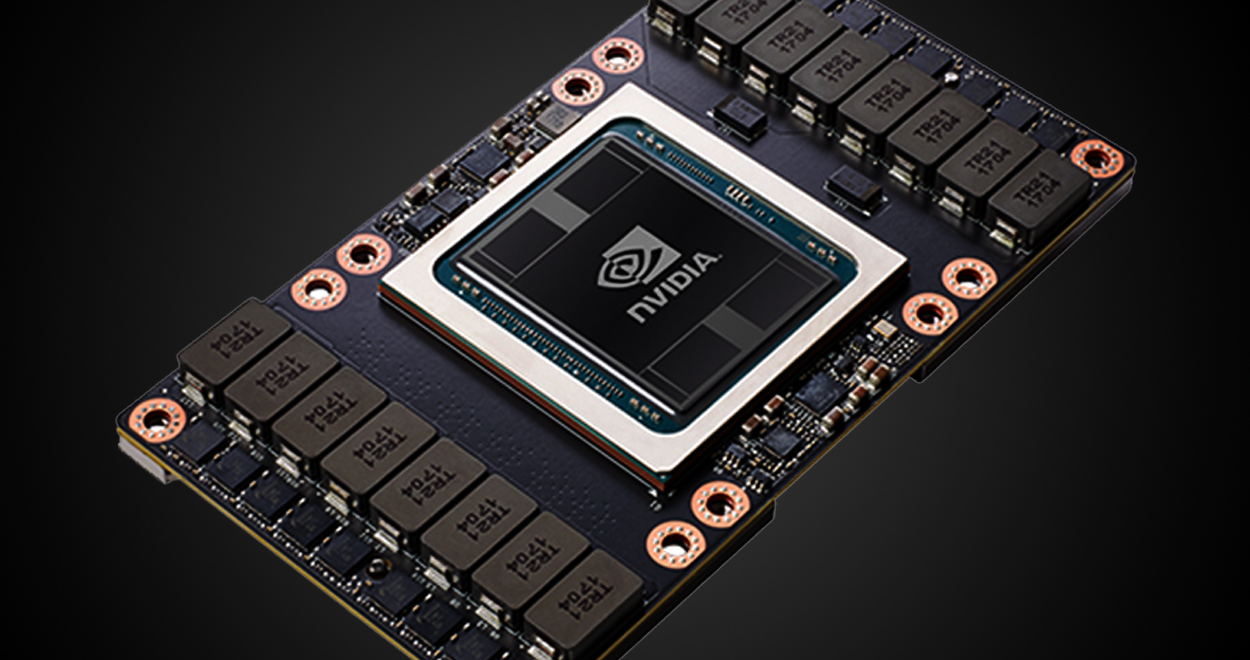
\includegraphics{images/V100.jpg}}

\date{\today}

\maketitle

\section{Motivation}

\begin{frame}{Motivation}
\framesubtitle{GPU-initiated Communication}

\vspace{1.3cm}
\begin{columns}[onlytextwidth,c]%ohne das c ist die Ausrichtung verschoben

	\column{.5\linewidth}
	
	\begin{figure}
	\centering
	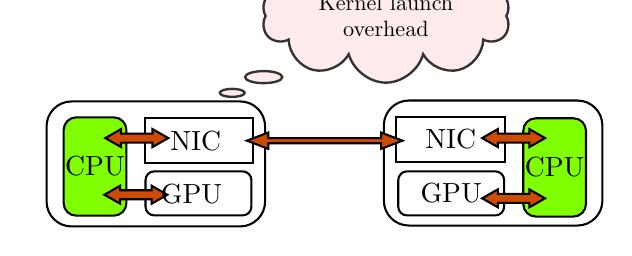
\begin{tikzpicture}[x=0.5pt,y=0.5pt,scale=0.65]
    \path (0,300); %set diagram left start at 0, and has height of 300

    %Rounded Rect [id:dp602011306068072] 
    \draw   (21,106.8) .. controls (21,91.45) and (33.45,79) .. (48.8,79) -- (236.2,79) .. controls (251.55,79) and (264,91.45) .. (264,106.8) -- (264,190.2)     .. controls (264,205.55) and (251.55,218) .. (236.2,218) -- (48.8,218) .. controls (33.45,218) and (21,205.55) .. (21,190.2) -- cycle ;
    %Rounded Rect [id:dp18758960033065608] 
    \draw   (396,107.8) .. controls (396,92.45) and (408.45,80) .. (423.8,80) -- (611.2,80) .. controls (626.55,80) and (639,92.45) .. (639,107.8) --     (639,191.2) .. controls (639,206.55) and (626.55,219) .. (611.2,219) -- (423.8,219) .. controls (408.45,219) and (396,206.55) .. (396,191.2) -- cycle ;
    %Rounded Rect [id:dp6120664204960634] 
    \draw   (40,104.95) .. controls (40,97.25) and (46.25,91) .. (53.95,91) -- (95.8,91) .. controls (103.5,91) and (109.75,97.25) .. (109.75,104.95) --     (109.75,186.3) .. controls (109.75,194) and (103.5,200.25) .. (95.8,200.25) -- (53.95,200.25) .. controls (46.25,200.25) and (40,194) .. (40,186.3) --     cycle [fill={rgb:green,1;yellow,1;pink,0}];
    %Rounded Rect [id:dp21812393541423936] 
    \draw   (551,103.95) .. controls (551,96.25) and (557.25,90) .. (564.95,90) -- (606.8,90) .. controls (614.5,90) and (620.75,96.25) .. (620.75,103.95) --     (620.75,185.3) .. controls (620.75,193) and (614.5,199.25) .. (606.8,199.25) -- (564.95,199.25) .. controls (557.25,199.25) and (551,193) .. (551,185.3)     -- cycle [fill={rgb:green,1;yellow,1;pink,0}] ;
    %Rounded Rect [id:dp5570992455242908] 
    \draw   (131,101.05) .. controls (131,95.64) and (135.39,91.25) .. (140.8,91.25) -- (238.95,91.25) .. controls (244.36,91.25) and (248.75,95.64) ..     (248.75,101.05) -- (248.75,130.45) .. controls (248.75,135.86) and (244.36,140.25) .. (238.95,140.25) -- (140.8,140.25) .. controls (135.39,140.25) and     (131,135.86) .. (131,130.45) -- cycle ;
    %Rounded Rect [id:dp9865384483688472] 
    \draw   (412,101.05) .. controls (412,95.64) and (416.39,91.25) .. (421.8,91.25) -- (519.95,91.25) .. controls (525.36,91.25) and (529.75,95.64) ..     (529.75,101.05) -- (529.75,130.45) .. controls (529.75,135.86) and (525.36,140.25) .. (519.95,140.25) -- (421.8,140.25) .. controls (416.39,140.25) and     (412,135.86) .. (412,130.45) -- cycle;
    %Shape: Rectangle [id:dp5183376461620953] 
    \draw   (130,150) -- (250.75,150) -- (250.75,199.25) -- (130,199.25) -- cycle ;
    %Shape: Rectangle [id:dp2368467260325865] 
    \draw   (410,151) -- (530.75,151) -- (530.75,200.25) -- (410,200.25) -- cycle ;
    %Left Right Arrow [id:dp5286461875079793] 
    \draw  [fill={rgb, 255:red, 204; green, 76; blue, 3 }  ,fill opacity=1 ] (85.3,114.25) -- (102.8,104.25) -- (102.8,109.25) -- (137.8,109.25) --     (137.8,104.25) -- (155.3,114.25) -- (137.8,124.25) -- (137.8,119.25) -- (102.8,119.25) -- (102.8,124.25) -- cycle ;
    %Left Right Arrow [id:dp2994575111375585] 
    \draw  [fill={rgb, 255:red, 204; green, 76; blue, 3 }  ,fill opacity=1 ] (505.3,110.25) -- (522.8,100.25) -- (522.8,105.25) -- (557.8,105.25) --     (557.8,100.25) -- (575.3,110.25) -- (557.8,120.25) -- (557.8,115.25) -- (522.8,115.25) -- (522.8,120.25) -- cycle ;
    %Left Right Arrow [id:dp9904840465412947] 
    \draw  [fill={rgb, 255:red, 204; green, 76; blue, 3 }  ,fill opacity=1 ] (243.75,174.35) -- (267.57,165.25) -- (267.57,171.53) -- (392.93,171.53) --     (392.93,165.25) -- (416.75,174.35) -- (392.93,183.45) -- (392.93,177.17) -- (267.57,177.17) -- (267.57,183.45) -- cycle ;
    %Left Right Arrow [id:dp47754037113398307] 
    \draw  [fill={rgb, 255:red, 204; green, 76; blue, 3 }  ,fill opacity=1 ] (86.3,177.25) -- (103.8,167.25) -- (103.8,172.25) -- (138.8,172.25) --     (138.8,167.25) -- (156.3,177.25) -- (138.8,187.25) -- (138.8,182.25) -- (103.8,182.25) -- (103.8,187.25) -- cycle ;
    %Left Right Arrow [id:dp7512448088396187] 
    \draw  [fill={rgb, 255:red, 204; green, 76; blue, 3 }  ,fill opacity=1 ] (505.3,177.25) -- (522.8,167.25) -- (522.8,172.25) -- (557.8,172.25) --     (557.8,167.25) -- (575.3,177.25) -- (557.8,187.25) -- (557.8,182.25) -- (522.8,182.25) -- (522.8,187.25) -- cycle ;

    \draw (74.88,145.63) node   [align=left] {CPU};
    \draw (585.88,144.63) node   [align=left] {CPU};
    \draw (182.25,115.5) node   [align=left] {GPU};
    \draw (470.88,115.75) node   [align=left] {GPU};
    \draw (186.92,174.5) node   [align=left] {NIC};
    \draw (470.38,175.63) node   [align=left] {NIC}; (image)
    \node<2->[overlay,cloud callout,callout relative pointer={(-1cm,-0.5cm)},aspect=3, align=center, line width=0.3mm, draw=black!80,  fill=red!8, scale=0.8] at (+7cm,+5.5cm) {Kernel launch\\overhead};
    \end{tikzpicture}
    \caption{CPU in critical path}
    \end{figure}
    
	\column{.5\linewidth}
	
	\begin{figure}
	    \centering
	    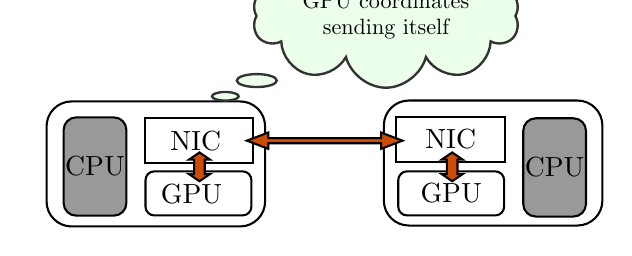
\begin{tikzpicture}[x=0.5pt,y=0.5pt,scale=0.65]
        \path (0,300); %set diagram left start at 0, and has height of 300

    %Rounded Rect [id:dp602011306068072] 
    \draw   (21,106.8) .. controls (21,91.45) and (33.45,79) .. (48.8,79) -- (236.2,79) .. controls (251.55,79) and (264,91.45) .. (264,106.8) -- (264,190.2)     .. controls (264,205.55) and (251.55,218) .. (236.2,218) -- (48.8,218) .. controls (33.45,218) and (21,205.55) .. (21,190.2) -- cycle ;
    %Rounded Rect [id:dp18758960033065608] 
    \draw   (396,107.8) .. controls (396,92.45) and (408.45,80) .. (423.8,80) -- (611.2,80) .. controls (626.55,80) and (639,92.45) .. (639,107.8) --     (639,191.2) .. controls (639,206.55) and (626.55,219) .. (611.2,219) -- (423.8,219) .. controls (408.45,219) and (396,206.55) .. (396,191.2) -- cycle ;
    %Rounded Rect [id:dp6120664204960634] 
    \draw   (40,104.95) .. controls (40,97.25) and (46.25,91) .. (53.95,91) -- (95.8,91) .. controls (103.5,91) and (109.75,97.25) .. (109.75,104.95) --     (109.75,186.3) .. controls (109.75,194) and (103.5,200.25) .. (95.8,200.25) -- (53.95,200.25) .. controls (46.25,200.25) and (40,194) .. (40,186.3) --     cycle [fill=black!40]; 
    %Rounded Rect [id:dp21812393541423936] 
    \draw   (551,103.95) .. controls (551,96.25) and (557.25,90) .. (564.95,90) -- (606.8,90) .. controls (614.5,90) and (620.75,96.25) .. (620.75,103.95) --     (620.75,185.3) .. controls (620.75,193) and (614.5,199.25) .. (606.8,199.25) -- (564.95,199.25) .. controls (557.25,199.25) and (551,193) .. (551,185.3)     -- cycle [fill=black!40];
    %Rounded Rect [id:dp5570992455242908] 
    \draw   (131,101.05) .. controls (131,95.64) and (135.39,91.25) .. (140.8,91.25) -- (238.95,91.25) .. controls (244.36,91.25) and (248.75,95.64) ..     (248.75,101.05) -- (248.75,130.45) .. controls (248.75,135.86) and (244.36,140.25) .. (238.95,140.25) -- (140.8,140.25) .. controls (135.39,140.25) and     (131,135.86) .. (131,130.45) -- cycle ;
    %Rounded Rect [id:dp9865384483688472] 
    \draw   (412,101.05) .. controls (412,95.64) and (416.39,91.25) .. (421.8,91.25) -- (519.95,91.25) .. controls (525.36,91.25) and (529.75,95.64) ..     (529.75,101.05) -- (529.75,130.45) .. controls (529.75,135.86) and (525.36,140.25) .. (519.95,140.25) -- (421.8,140.25) .. controls (416.39,140.25) and     (412,135.86) .. (412,130.45) -- cycle ;
    %Shape: Rectangle [id:dp5183376461620953] 
    \draw   (130,150) -- (250.75,150) -- (250.75,199.25) -- (130,199.25) -- cycle ;
    %Shape: Rectangle [id:dp2368467260325865] 
    \draw   (410,151) -- (530.75,151) -- (530.75,200.25) -- (410,200.25) -- cycle ;
    %Left Right Arrow [id:dp9904840465412947] 
    \draw  [fill={rgb, 255:red, 204; green, 76; blue, 3 }  ,fill opacity=1 ] (243.75,174.35) -- (267.57,165.25) -- (267.57,171.53) -- (392.93,171.53) --     (392.93,165.25) -- (416.75,174.35) -- (392.93,183.45) -- (392.93,177.17) -- (267.57,177.17) -- (267.57,183.45) -- cycle ;
    %Left Right Arrow [id:dp47754037113398307] 
    \draw  [fill={rgb, 255:red, 204; green, 76; blue, 3 }  ,fill opacity=1 ] (191.03,129.25) -- (202.75,137.25) -- (196.89,137.25) -- (196.89,153.25) --     (202.75,153.25) -- (191.03,161.25) -- (179.3,153.25) -- (185.16,153.25) -- (185.16,137.25) -- (179.3,137.25) -- cycle ;
    %Left Right Arrow [id:dp2871368640426972] 
    \draw  [fill={rgb, 255:red, 204; green, 76; blue, 3 }  ,fill opacity=1 ] (472.03,129.25) -- (483.75,137.25) -- (477.89,137.25) -- (477.89,153.25) --     (483.75,153.25) -- (472.03,161.25) -- (460.3,153.25) -- (466.16,153.25) -- (466.16,137.25) -- (460.3,137.25) -- cycle ;
    
    % Text Node
    \draw (74.88,145.63) node   [align=left] {CPU};
    % Text Node
    \draw (585.88,144.63) node   [align=left] {CPU};
    % Text Node
    \draw (182.25,115.5) node   [align=left] {GPU};
    % Text Node
    \draw (470.88,115.75) node   [align=left] {GPU};
    % Text Node
    \draw (186.92,174.5) node   [align=left] {NIC};
    % Text Node
    \draw (470.38,175.63) node   [align=left] {NIC};
    
     (image)
        \node<3->[overlay,cloud callout,callout relative pointer={(-1cm,-0.5cm)},aspect=3, align=center, line width=0.3mm, draw=black!80,  fill=green!8, scale=0.8] at (+7cm,+5.5cm) {GPU coordinates\\sending itself};
    \end{tikzpicture}
    \caption{CPU out of critical path}
	\end{figure}
	
\end{columns}

\end{frame}

%\begin{frame}{The Critical Path - Motivation}

% This text has been explained on previous slide, do not put it on this slide
% Common GPU programming idiom involves launching compute-heavy kernels on Device (GPU) and returning control to Host (CPU) before next kernel is launched - CPU is in critical path 

%\vbaselineskip

%\begin{alertblock}{Issue}
%Repeated kernel launches introduce a calling overhead and impeding scaling 
%\end{alertblock}

%\begin{exampleblock}{Idea}
%Take CPU out of the critical path and initiate network transfer from GPU    
%\end{exampleblock}

%\end{frame}

\begin{frame}{Motivation}
\framesubtitle{Kernel Launch Overhead}

\begin{center}
\begin{tikzpicture}
\centering
\node[anchor=south west,inner sep=0](image) at(0,0){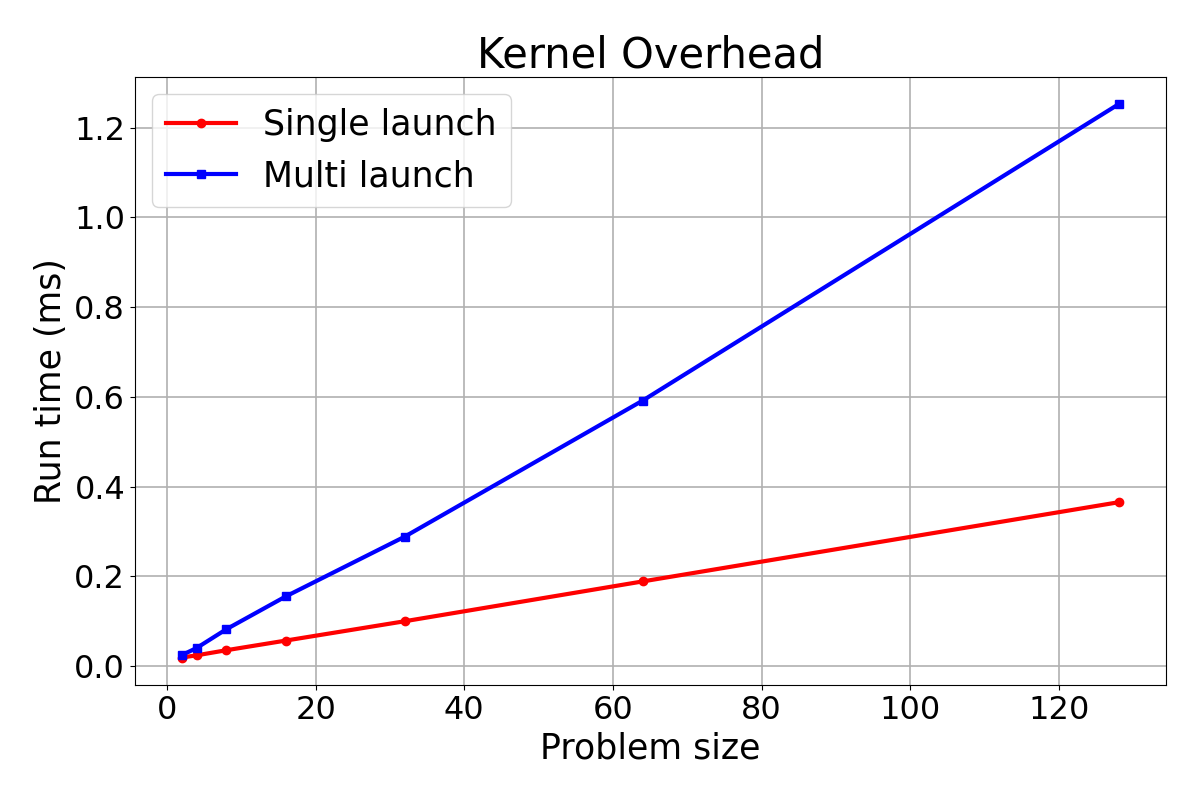
\includegraphics[width=0.6\textwidth]{images/overhead.png}};

        \node<2->[overlay,cloud callout,callout relative pointer={(-1.5cm,-0.8cm)}, line width=0.3mm, draw=black!80,  fill=black!8, aspect=3, align=center, scale=0.8] at ($(image.center)+(+5cm,+2cm)$) {Kernel launches are not free};%

\end{tikzpicture}
\end{center} 

\end{frame}

\section{Outline}

\begin{frame}{Outline}
\begin{itemize}
    \item Motivation
    \item Use Case: Distributed Shuffle
    \item Microbenchmarks and Implementation
    \item Evaluation
    \item Conclusion
\end{itemize}
\end{frame}


\section{Background}

\begin{frame}{Use Case}
\framesubtitle{Distributed Shuffle}

\begin{itemize}
    \item Join requires same keys on same node
\end{itemize}

\begin{figure}
    \centering
    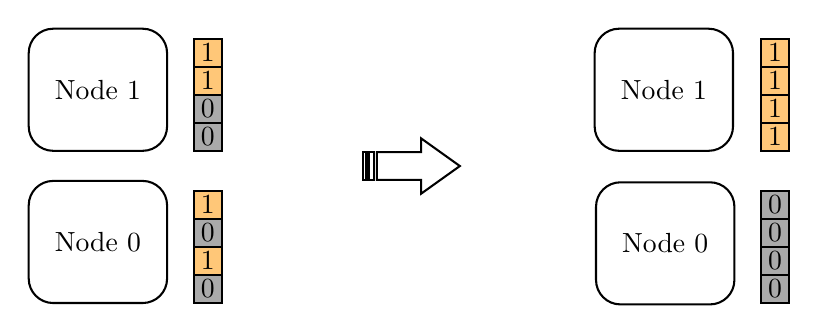
\begin{tikzpicture}[x=0.5pt,y=0.5pt,scale=1]
        %uncomment if require: \path (0,300); %set diagram left start at 0, and has height of 300

%Rounded Rect [id:dp6258266303889986] 
\draw   (21.42,78.65) .. controls (21.42,68.9) and (29.32,61) .. (39.07,61) -- (103.77,61) .. controls (113.51,61) and (121.42,68.9) .. (121.42,78.65) -- (121.42,131.6) .. controls (121.42,141.35) and (113.51,149.25) .. (103.77,149.25) -- (39.07,149.25) .. controls (29.32,149.25) and (21.42,141.35) .. (21.42,131.6) -- cycle ;
%Rounded Rect [id:dp4329118115958088] 
\draw   (21.42,188.65) .. controls (21.42,178.9) and (29.32,171) .. (39.07,171) -- (103.77,171) .. controls (113.51,171) and (121.42,178.9) .. (121.42,188.65) -- (121.42,241.6) .. controls (121.42,251.35) and (113.51,259.25) .. (103.77,259.25) -- (39.07,259.25) .. controls (29.32,259.25) and (21.42,251.35) .. (21.42,241.6) -- cycle ;
%Rounded Rect [id:dp015597904001152796] 
\draw   (431.42,77.65) .. controls (431.42,67.9) and (439.32,60) .. (449.07,60) -- (513.77,60) .. controls (523.51,60) and (531.42,67.9) .. (531.42,77.65) -- (531.42,130.6) .. controls (531.42,140.35) and (523.51,148.25) .. (513.77,148.25) -- (449.07,148.25) .. controls (439.32,148.25) and (431.42,140.35) .. (431.42,130.6) -- cycle ;
%Rounded Rect [id:dp9157348285554725] 
\draw   (430.42,188.65) .. controls (430.42,178.9) and (438.32,171) .. (448.07,171) -- (512.77,171) .. controls (522.51,171) and (530.42,178.9) .. (530.42,188.65) -- (530.42,241.6) .. controls (530.42,251.35) and (522.51,259.25) .. (512.77,259.25) -- (448.07,259.25) .. controls (438.32,259.25) and (430.42,251.35) .. (430.42,241.6) -- cycle ;
%Shape: Square [id:dp4905173723281211] 
\draw   (140.75,61) -- (161,61) -- (161,81.25) -- (140.75,81.25) -- cycle [fill={rgb:black,1;white,2}] ;
%Shape: Square [id:dp8440688980415447] 
\draw   (140.75,81.25) -- (161,81.25) -- (161,101.5) -- (140.75,101.5) -- cycle [fill={rgb:orange,1;yellow,2;pink,5}];
%Shape: Square [id:dp7458380895324004] 
\draw   (140.75,101.5) -- (161,101.5) -- (161,121.75) -- (140.75,121.75) -- cycle [fill={rgb:black,1;white,2}];
%Shape: Square [id:dp058354526525468575] 
\draw   (140.75,121.75) -- (161,121.75) -- (161,142) -- (140.75,142) -- cycle [fill={rgb:orange,1;yellow,2;pink,5}];
%Shape: Square [id:dp18391666551702146] 
\draw   (140.75,171) -- (161,171) -- (161,191.25) -- (140.75,191.25) -- cycle [fill={rgb:black,1;white,2}];
%Shape: Square [id:dp6120784512538862] 
\draw   (140.75,191.25) -- (161,191.25) -- (161,211.5) -- (140.75,211.5) -- cycle [fill={rgb:black,1;white,2}];
%Shape: Square [id:dp8747397824735408] 
\draw   (140.75,211.5) -- (161,211.5) -- (161,231.75) -- (140.75,231.75) -- cycle [fill={rgb:orange,1;yellow,2;pink,5}];
%Shape: Square [id:dp5766436844029047] 
\draw   (140.75,231.75) -- (161,231.75) -- (161,252) -- (140.75,252) -- cycle [fill={rgb:orange,1;yellow,2;pink,5}];
%Shape: Square [id:dp6395405576891373] 
\draw   (550.75,61) -- (571,61) -- (571,81.25) -- (550.75,81.25) -- cycle [fill={rgb:black,1;white,2}];
%Shape: Square [id:dp3329077106272186] 
\draw   (550.75,81.25) -- (571,81.25) -- (571,101.5) -- (550.75,101.5) -- cycle [fill={rgb:black,1;white,2}];
%Shape: Square [id:dp998173598921265] 
\draw   (550.75,101.5) -- (571,101.5) -- (571,121.75) -- (550.75,121.75) -- cycle [fill={rgb:black,1;white,2}];
%Shape: Square [id:dp379654712623825] 
\draw   (550.75,121.75) -- (571,121.75) -- (571,142) -- (550.75,142) -- cycle [fill={rgb:black,1;white,2}];
%Shape: Square [id:dp8814370523523429] 
\draw   (550.75,171) -- (571,171) -- (571,191.25) -- (550.75,191.25) -- cycle [fill={rgb:orange,1;yellow,2;pink,5}];
%Shape: Square [id:dp03771997443662467] 
\draw   (550.75,191.25) -- (571,191.25) -- (571,211.5) -- (550.75,211.5) -- cycle [fill={rgb:orange,1;yellow,2;pink,5}];
%Shape: Square [id:dp31920370442327983] 
\draw   (550.75,211.5) -- (571,211.5) -- (571,231.75) -- (550.75,231.75) -- cycle [fill={rgb:orange,1;yellow,2;pink,5}];
%Shape: Square [id:dp33663607824004405] 
\draw   (550.75,231.75) -- (571,231.75) -- (571,252) -- (550.75,252) -- cycle [fill={rgb:orange,1;yellow,2;pink,5}];
%Striped Right Arrow [id:dp7696802111282792] 
\draw   (273,150) -- (305,150) -- (305,140) -- (333,160) -- (305,180) -- (305,170) -- (273,170) -- cycle ;\draw   (263,150) -- (265,150) -- (265,170) -- (263,170) -- cycle ;\draw   (267,150) -- (271,150) -- (271,170) -- (267,170) -- cycle ;

% Text Node
\draw (71.42,105.13) node   [align=left] {Node 0};
% Text Node
\draw (481.42,104.13) node   [align=left] {Node 0};
% Text Node
\draw (71.42,215.13) node   [align=left] {Node 1};
% Text Node
\draw (480.42,215.13) node   [align=left] {Node 1};
% Text Node
\draw (150.88,71.13) node   [align=left] {0};
% Text Node
\draw (150.88,111.63) node   [align=left] {0};
% Text Node
\draw (150.88,181.13) node   [align=left] {0};
% Text Node
\draw (150.88,201.38) node   [align=left] {0};
% Text Node
\draw (560.88,71.13) node   [align=left] {0};
% Text Node
\draw (560.88,91.38) node   [align=left] {0};
% Text Node
\draw (560.88,111.63) node   [align=left] {0};
% Text Node
\draw (560.88,131.88) node   [align=left] {0};
% Text Node
\draw (150.88,91.38) node   [align=left] {1};
% Text Node
\draw (150.88,131.88) node   [align=left] {1};
% Text Node
\draw (150.88,221.63) node   [align=left] {1};
% Text Node
\draw (150.88,241.88) node   [align=left] {1};
% Text Node
\draw (560.88,181.13) node   [align=left] {1};
% Text Node
\draw (560.88,201.38) node   [align=left] {1};
% Text Node
\draw (560.88,221.63) node   [align=left] {1};
% Text Node
\draw (560.88,241.88) node   [align=left] {1};
% Text Node
%\draw (243,117) node [anchor=north west][inner sep=0.75pt]   [align=left] {Shuffle operation};
    \end{tikzpicture}

    \caption{Principle idea of shuffling}
\end{figure}

% JW: suggestion for points to be delivered with this slide:
% - In a dist. database system, tuples are distributed among the nodes -> each server has a partition of the total data
% - Common and expensive (critical) DB operation is joining (finding tuples based on an equality comparison on a given column (join key))
% - To find join partners, the tuples must be located on the same server. If they are not, they must be send over the network -> this is called shuffling.
% - modern databases use partitioning schemes like hash partitioning, trying to locate possible join partners on the same machine. But this is only possible for one column -> Avoiding shuffling completely not possible.
% - Shuffle input on each server: [(randomly) distributed tuples, join column]
% - Shuffle output on each server: [for a part of the key space, all tuples having this key (including tuples that initially have been stored remotely)]
% - Output of shuffle is input to a -local- join operator

% We could think of a figure describing the above. First idea:
% 2 Servers on left (rectangles), next to them 3 tuples each. Their join key should be clearly visible. To make it more illustrative, we could use a symbol (star, circle, rectangle, triangle) instead of numbers for the join key.
% 2 servers on the right (the same servers but shown again on the right for better visibility)
% left servers send (shown by arrows) tuples with same join key (symbol) to same server on the right side.
% next to the servers on the right side, the result distribution of the tuples is shown

% At some point, we have to go over the most important shuffle implementation. But this fits probably better into the section "implementation" since it will be more detailed. This slide should probably only convey a simple impression of what a shuffle is 

\end{frame}


\section{GPU-Initiated Shuffle}

% \begin{frame}[c]{GPU-Initiated Shuffle}
% \framesubtitle{Design Challenges: Balance network and compute?}
%     \centering
%     \begin{tikzpicture}
%         \node[cpu] (cpu-0) {CPU};
%         \node[gpu, below left=0.5em and -3.75em of cpu-0] (gpu-0) {GPU};
%         \node[nic, below right=0.5em and -3.75em of cpu-0] (nic-0) {NIC};
%         \node[node-box, fit=(cpu-0) (gpu-0) (nic-0), label={[font=\small, align=center, text width=4em]above:Node}] (node-0) {};
    
%         \draw[double, thick, latex'-latex'] ([xshift=1em]node-0.east)
%         -- node [near end, right=2em] {Network}
%         ([xshift=5em]node-0.east);
        
%         \node<2>[cpu, fill=TUDa-9b] (cpu-1) {CPU};
        
%         \node<2>[overlay,cloud callout,callout relative pointer={(-1cm,-2cm)},aspect=3, line width=0.3mm, draw=black!80,  fill=black!8, scale=0.5] at ($(cpu-1.center)+(+2cm,+2cm)$) {Help! I'm overloaded!};
        
%         \node<3>[nic, below right=0.5em and -3.75em of cpu-0, fill=TUDa-9b] (nic-1) {NIC};
        
%         \draw<3>[double, thick, latex'-latex', draw=TUDa-9b] ([xshift=1em]node-0.east)
%         -- node [near end, right=2em, text=TUDa-9b] {Network}
%         ([xshift=5em]node-0.east);
        
%         \node<3>[overlay,cloud callout,callout relative pointer={(-1cm,-2cm)},aspect=3, line width=0.3mm, draw=black!80,  fill=black!8, scale=0.5] at ($(node-0.east)+(+4cm,+2cm)$) {Help! I'm overloaded!};
%     \end{tikzpicture}
% \end{frame}


\begin{frame}[c]{GPU-Initiated Shuffle}
    \framesubtitle{Design Challenges}
    \centering
    % \node[anchor=south west,inner sep=0](image) at(0,0){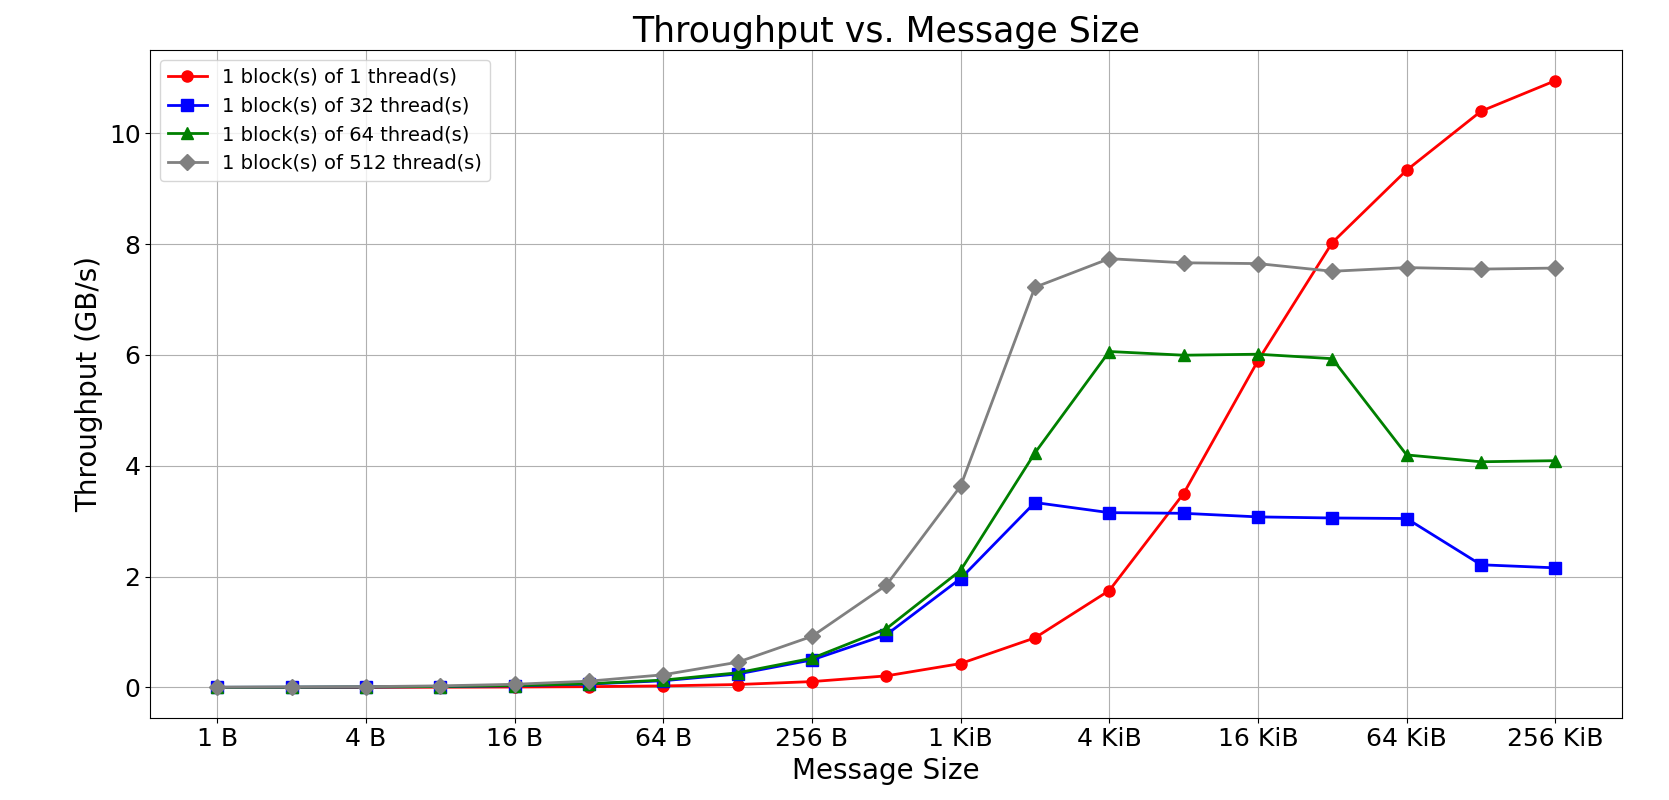
\includegraphics[width=0.7\textwidth]{images/put_granularity_grid1.png}};
    
    \begin{tikzpicture}
        \node (image) {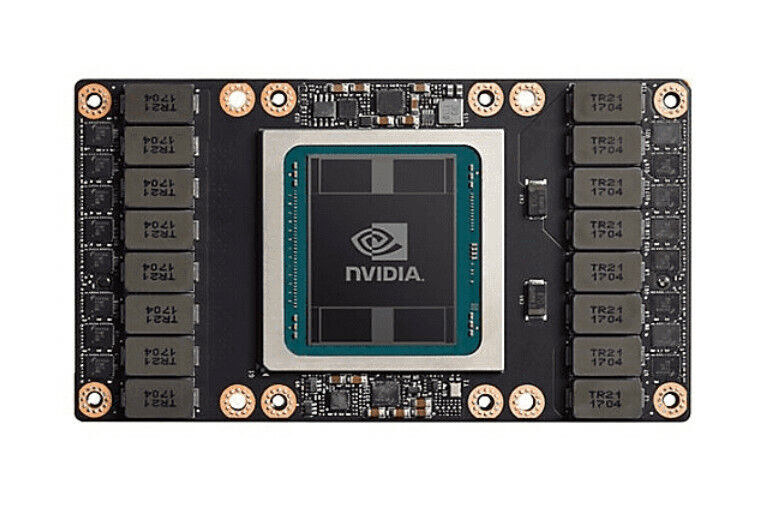
\includegraphics[width=.7\textwidth]{images/gpu.png}};
        
        % Draw eyes
        \fill[white] (image.center) ++(-0.6,1) circle (0.2);
        \fill[white] (image.center) ++(0.6,1) circle (0.2);
        
        \fill<1>[black] (image.center) ++(-0.6,0.95) circle (0.1);
        \fill<1>[black] (image.center) ++(0.6,0.95) circle (0.1);
        
        % Draw mouth with a smile
        \draw[red, line width=2pt] (image.center) ++(-0.4,-0.8) arc [start angle=-170, end angle=-10, radius=0.4];
        
        \fill<2>[black] (image.center) ++(-0.55,1.05) circle (0.1);
        \fill<2>[black] (image.center) ++(0.65,1.05) circle (0.1);
        
        \node<2>[overlay,cloud callout,callout relative pointer={(-1cm,-2cm)},aspect=3, line width=0.3mm, draw=black!80,  fill=black!8, scale=0.8, align=center] at ($(image.center)+(+2cm,+4cm)$) {Coordination\\of remote memory?};


    \end{tikzpicture}
\end{frame}

\begin{frame}[c]{Shuffle Implementation}
    \framesubtitle{Remote Write Offsets}
    % Maybe a figure or sequence of figures that describe the previous text slide?
    \begin{tikzpicture}
    \node[data-box](data-box-0){2};
    \node[data-box, below=0em of data-box-0](data-box-1){3};
    \node[data-box, below=0em of data-box-1](data-box-2){4};
    \node[data-box, below=0em of data-box-2](data-box-3){5};
    \node[data-box, below=0em of data-box-3](data-box-4){6};
    \node[data-box, below=0em of data-box-4](data-box-5){7};
    \node[data-box, below=0em of data-box-5](data-box-6){8};
    \node[data-box, below=0em of data-box-6](data-box-7){9};
    
    \draw[dotted, thick, -Latex] ([yshift=-0.25em]data-box-7.south)
    -- ([yshift=-2em]data-box-7.south);
    \draw[dotted, thick, -Latex] ([yshift=0.25em]data-box-0.north)
    -- ([yshift=2em]data-box-0.north);
    
    % Histogram Node 1
    \node[hist-box, right=8em of data-box-2](hist-0-0){3};
    \node[anchor=south east,inner sep=2pt, text=TUDa-4d] at (hist-0-0.south east){\footnotesize$\rightarrow 0$};

    \node[hist-box, below=0em of hist-0-0](hist-0-1){2};
    \node[anchor=south east,inner sep=2pt, text=TUDa-4d] at (hist-0-1.south east){\footnotesize$\rightarrow 1$};

    \node[hist-box, below=0em of hist-0-1](hist-0-2){3};
    \node[anchor=south east,inner sep=2pt, text=TUDa-4d] at (hist-0-2.south east){\footnotesize$\rightarrow 2$};
    
    % Create invisible hist-0-2 box for fit
    \node[hist-box, below=3em of hist-0-0, opacity=0](hist-0-final){};
    
    \node[hist-buf, fit=(hist-0-0) (hist-0-final), label={[text=TUDa-4d, font=\small, align=center, text width=4em]above:Local\\Histogram Node 0}] (hist-buf-0-box) {};
    
    % Animated arrows
    % Yes, this should probably be done with custom commands to avoid repetition
    \draw<1>[thick, -Latex] (data-box-0.east) -- (hist-0-2.west) {};
    \draw<2->[thick, -Latex, opacity=0.15] (data-box-0.east) -- (hist-0-2.west) {};

    \draw<1>[thick, -Latex] (data-box-1.east) -- (hist-0-0.west) {};
    \draw<2->[thick, -Latex, opacity=0.15] (data-box-1.east) -- (hist-0-0.west) {};

    \draw<1>[thick, -Latex] (data-box-2.east) -- (hist-0-1.west) {};
    \draw<2->[thick, -Latex, opacity=0.15] (data-box-2.east) -- (hist-0-1.west) {};

    \draw<1>[thick, -Latex] (data-box-3.east) -- (hist-0-2.west) {};
    \draw<2->[thick, -Latex, opacity=0.15] (data-box-3.east) -- (hist-0-2.west) {};

    \draw<1>[thick, -Latex] (data-box-4.east) -- (hist-0-0.west) {};
    \draw<2->[thick, -Latex, opacity=0.15] (data-box-4.east) -- (hist-0-0.west) {};

    \draw<1>[thick, -Latex] (data-box-5.east) -- (hist-0-1.west) {};
    \draw<2->[thick, -Latex, opacity=0.15] (data-box-5.east) -- (hist-0-1.west) {};

    \draw<1>[thick, -Latex] (data-box-6.east) -- (hist-0-2.west) {};
    \draw<2->[thick, -Latex, opacity=0.15] (data-box-6.east) -- (hist-0-2.west) {};

    \draw<1>[thick, -Latex] (data-box-7.east) -- (hist-0-0.west) {};
    \draw<2->[thick, -Latex, opacity=0.15] (data-box-7.east) -- (hist-0-0.west) {};

    % Histogram Node 1
    
    \node<2->[hist-box, right=4em of hist-0-0](hist-1-0){$h_1(0)$};
    \node<2->[anchor=south east,inner sep=2pt, text=TUDa-4d] at (hist-1-0.south east){\footnotesize$\rightarrow 0$};

    \node<2->[hist-box, below=0em of hist-1-0](hist-1-1){$h_1(1)$};
    \node<2->[anchor=south east,inner sep=2pt, text=TUDa-4d] at (hist-1-1.south east){\footnotesize$\rightarrow 1$};

    \node<2->[hist-box, below=0em of hist-1-1](hist-1-2){$h_1(2)$};
    \node<2->[anchor=south east,inner sep=2pt, text=TUDa-4d] at (hist-1-2.south east){\footnotesize$\rightarrow 2$};
    
    \node<2->[hist-buf, fit=(hist-1-0) (hist-1-2), label={[text=TUDa-4d, font=\small, align=center, text width=4em]above:Local\\Histogram Node 1}] (hist-buf-1-box) {};
    
    % Histogram Node 2
    
    \node<2->[hist-box, right=4em of hist-1-0](hist-2-0){$h_2(0)$};
    \node<2->[anchor=south east,inner sep=2pt, text=TUDa-4d] at (hist-2-0.south east){\footnotesize$\rightarrow 0$};

    \node<2->[hist-box, below=0em of hist-2-0](hist-2-1){$h_2(1)$};
    \node<2->[anchor=south east,inner sep=2pt, text=TUDa-4d] at (hist-2-1.south east){\footnotesize$\rightarrow 1$};

    \node<2->[hist-box, below=0em of hist-2-1](hist-2-2){$h_2(2)$};
    \node<2->[anchor=south east,inner sep=2pt, text=TUDa-4d] at (hist-2-2.south east){\footnotesize$\rightarrow 2$};
    
    \node<2->[hist-buf, fit=(hist-2-0) (hist-2-2), label={[text=TUDa-4d, font=\small, align=center, text width=4em]above:Local\\Histogram Node 2}] (hist-buf-2-box) {};
    
    % Giant fcollect

    \coordinate<2-> (a) at ([yshift=-3em]hist-0-2.south);
    \coordinate<2-> (b) at ([yshift=-3em]hist-2-2.south);
    \coordinate<2-> (midpoint) at ($(a)!0.5!(b)$);

    \node<2->[single arrow, very thick, fill=TUDa-4d,
          minimum width=8pt, single arrow head extend=3pt,
          inner xsep=0pt,
          fit=(a) (b)] (arrow1) {};

    \node<2->[single arrow, very thick, fill=TUDa-4d,
          minimum width=8pt, single arrow head extend=3pt,
          inner xsep=0pt, rotate=180,
          fit=(a) (b)] (arrow2) {};
          
    \node<2->[above=1mm of midpoint, font=\footnotesize, text=TUDa-4d] {Exchange with fcollect};
    
    % Final Histogram
    
    \draw<3->[double, thick, -Latex] ([xshift=2em]hist-2-1.east)
    -- ([xshift=4em]hist-2-1.east);
    
    \node<3->[hist-box, minimum width=7em, right=6em of hist-2-0](hist-2-0){$\sum_{i=0}^{k-1} h_i(0)$};
    \node<3->[anchor=south east,inner sep=2pt, text=TUDa-4d] at (hist-2-0.south east){\footnotesize$\rightarrow 0$};
    
    \node<3->[hist-box, minimum width=7em, below=0em of hist-2-0](hist-2-1){$\sum_{i=0}^{k-1} h_i(1)$};
    \node<3->[anchor=south east,inner sep=2pt, text=TUDa-4d] at (hist-2-1.south east){\footnotesize$\rightarrow 1$};
    
    \node<3->[hist-box, minimum width=7em, below=0em of hist-2-1](hist-2-2){$\sum_{i=0}^{k-1} h_i(2)$};
    \node<3->[anchor=south east,inner sep=2pt, text=TUDa-4d] at (hist-2-2.south east){\footnotesize$\rightarrow 2$};
    
    \node<3->[hist-buf, fit=(hist-2-0) (hist-2-2), label={[text=TUDa-4d, font=\small, align=center, text width=4em]above:Offsets\\Node k}] (hist-buf-2-box) {};

\end{tikzpicture}
\end{frame}

\begin{frame}[c]{GPU-Initiated Shuffle}
\framesubtitle{Design Challenges}
    \centering
    \begin{tikzpicture}
        \node (image) {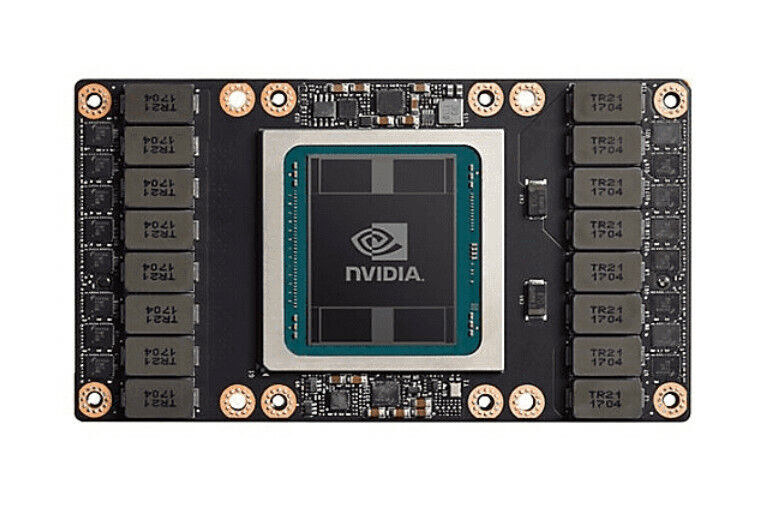
\includegraphics[width=.7\textwidth]{images/gpu.png}};
    
        % Draw eyes
        \fill[white] (image.center) ++(-0.6,1) circle (0.2);
        \fill[white] (image.center) ++(0.6,1) circle (0.2);
        
        \fill<1>[black] (image.center) ++(-0.65,1.05) circle (0.1);
        \fill<1>[black] (image.center) ++(0.55,1.05) circle (0.1);
        
        % Draw mouth with a smile
        \draw[red, line width=2pt] (image.center) ++(-0.4,-0.8) arc [start angle=-170, end angle=-10, radius=0.4];
        
        \node<1>[overlay,cloud callout,callout relative pointer={(1cm,-2cm)},aspect=3, line width=0.3mm, draw=black!80,  fill=black!8, scale=0.8, align=center] at ($(image.center)+(-2cm,+4cm)$) {Parallel sending?};
        
        \fill<2>[black] (image.center) ++(-0.55,1.05) circle (0.1);
        \fill<2>[black] (image.center) ++(0.65,1.05) circle (0.1);
        
        \node<2>[overlay,cloud callout,callout relative pointer={(-1cm,-2cm)},aspect=3, line width=0.3mm, draw=black!80,  fill=black!8, scale=0.8, align=center] at ($(image.center)+(+2cm,+4cm)$) {Frequency of sending?};
    \end{tikzpicture}
\end{frame}

% --- before meeting ---
% JW: things to be delivered using this slide:
% - To utilize computation and network capacity optimally, we want to compute and transmit previously computed data continually.
% - If we compute all the tuple's destination node ids in the first phase and then send the tuples in the second phase, we would leave network idle in the first phase and compute idle in the second stage -> not optimal
% - Instead we want to transmit tuples more often to have the computation of tuples of batch i overlap with the transmission of tuples of batch i-1
% CPU initiated shuffling would require one kernel launch per batch -> hypothesis: this has high overhead. We can show the kernel-launch-overhead-benchmark results here (if it hopefully shows that there is indeed some overhead)
% GPU initiated shuffling: allows to initiate asynchronous send operations from inside the kernel, making it possible to overlap computation and transmission with only a single kernel.

\section{Microbenchmarks and Implementation}

\begin{frame}{CPU- vs GPU-initiated RDMA performance}
    \centering
    \begin{tikzpicture}
        \node[anchor=south west,inner sep=0](image) at(0,0){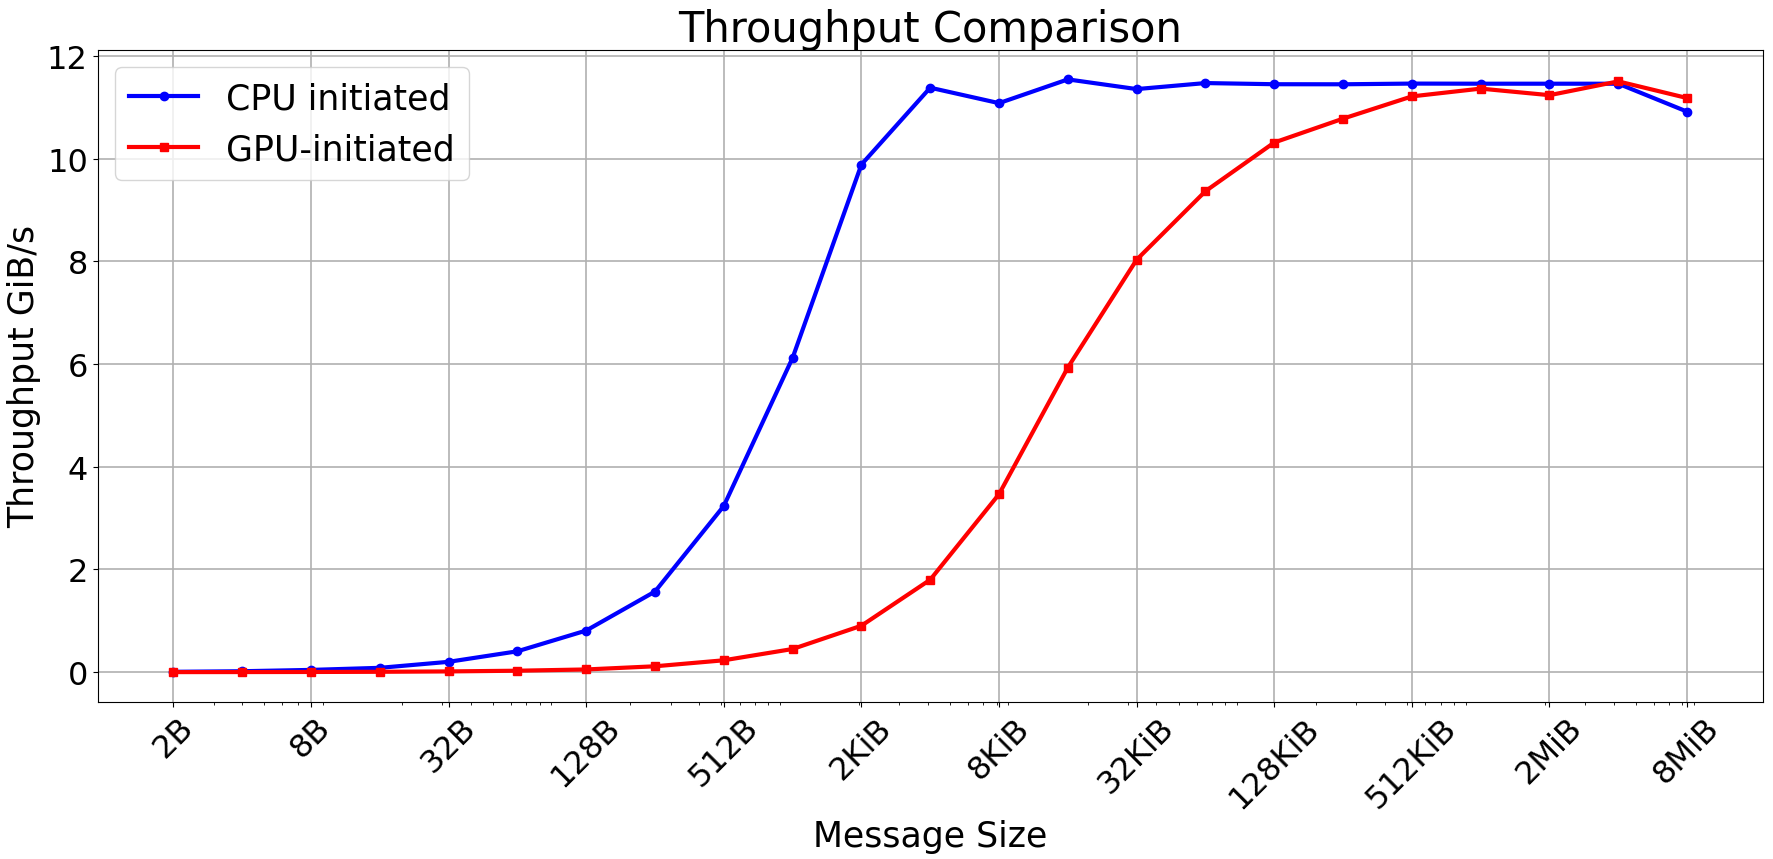
\includegraphics[width=0.8\textwidth]{images/09_gpu_cpu_st.png}};
        \node<2->[overlay,cloud callout,callout relative pointer={(-1.5cm,-0.8cm)}, line width=0.3mm, draw=black!80,  fill=black!8, aspect=3, align=center, scale=0.8] at ($(image.center)+(+3.5cm,+0.5cm)$) {GPU needs larger\\message size};
    \end{tikzpicture}
\end{frame}

\begin{frame}{Microbenchmarks}
    \framesubtitle{Async Sending with Grid Size 1}
    
    % Speaker:
    % - too small send sizes make no sense -> NVSHMEM does not buffer calls in background -> we should buffer before sending
    % - Sending with one thread gives the best performance, multiple threads make things worse
    % - performance drops again if send size too large, maybe some TLB caching issue
    % - When having non-aligned accesses, performance is very off
    % - -> non-trivial performance charactersistics
    
    \centering
    \begin{tikzpicture}
        \node[anchor=south west,inner sep=0](image) at(0,0){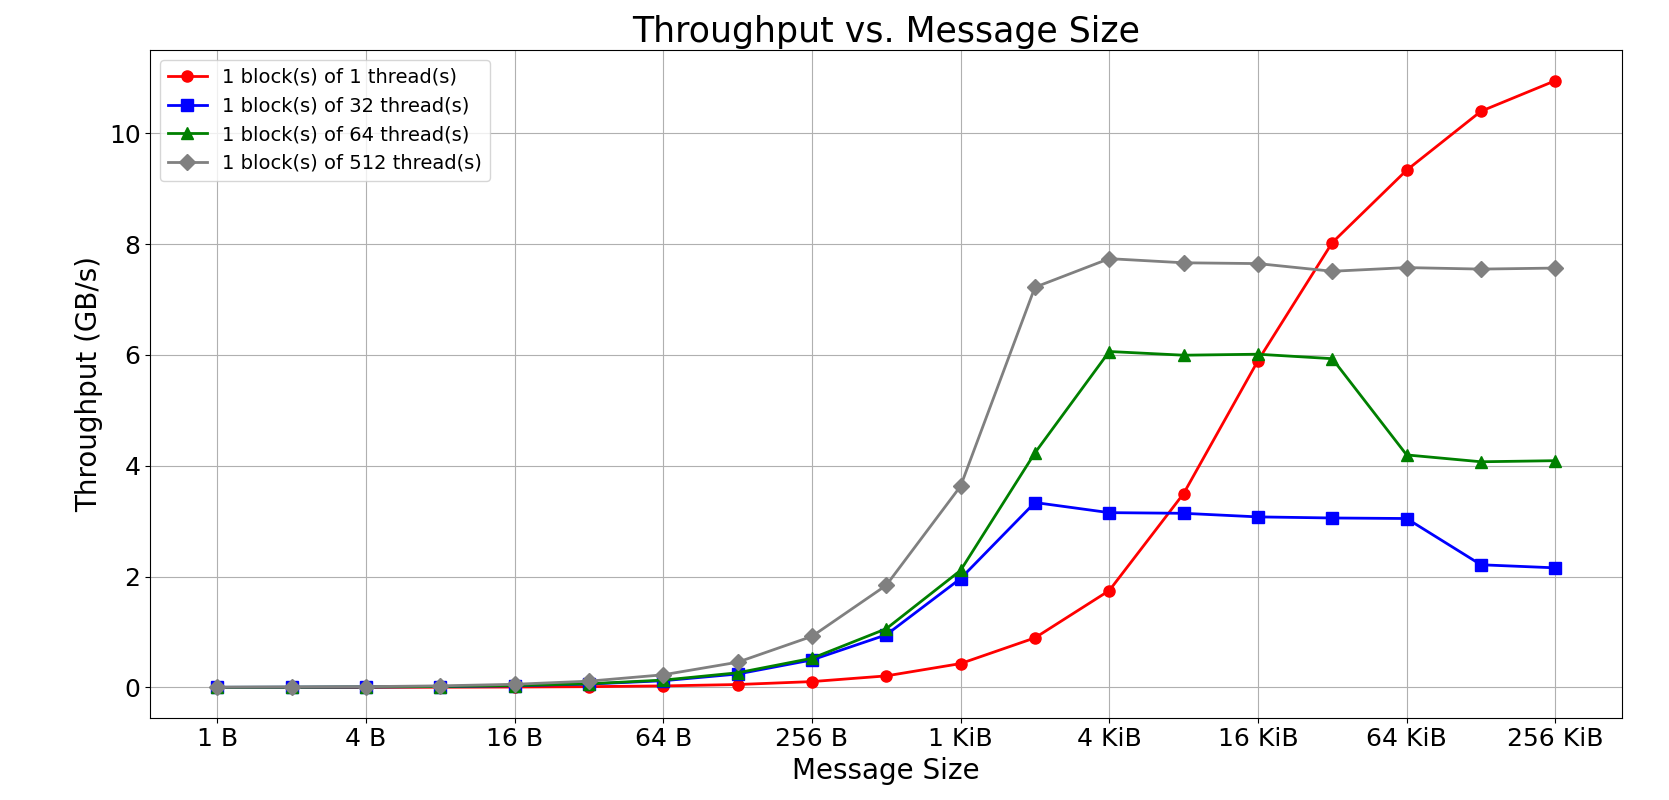
\includegraphics[width=0.7\textwidth]{images/put_granularity_grid1.png}};
        \node<2->[overlay,cloud callout,callout relative pointer={(-1cm,-2cm)},aspect=3, line width=0.3mm, draw=black!80,  fill=black!8, scale=0.8] at ($(image.center)+(+5cm,+2cm)$) {What about more blocks?};
    \end{tikzpicture}
\end{frame}

% Speaker:
% - When increasing the grid size, it is better to send with more threads
% -> performance not easy to understand
% -> Should use one of the configurations that is giving us 12.5 GB/s

\begin{frame}{Microbenchmarks}
    \framesubtitle{Async Sending with Grid Size 40}
    \vspace{-5.0\lineheight}
    \centering
    \begin{tikzpicture}
        \node[anchor=south west,inner sep=0] at(0,0){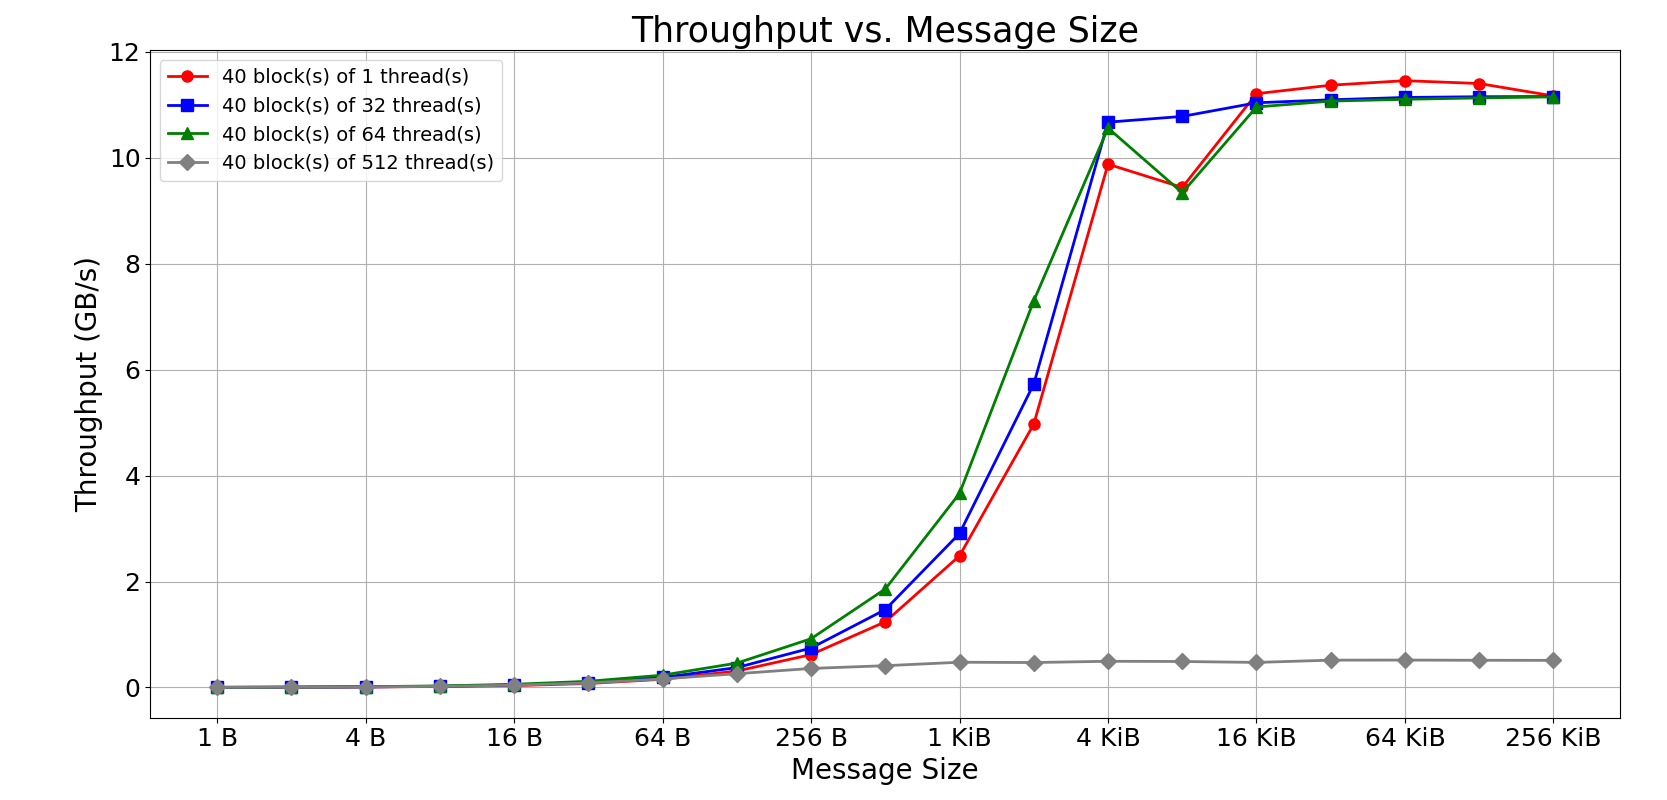
\includegraphics[width=0.7\textwidth]{images/put_granularity_grid40.png}};
        \node<2->[overlay,cloud callout,callout relative pointer={(-3.1cm,-2cm)},aspect=3, align=center, line width=0.3mm, draw=black!80,  fill=black!8, scale=0.8] at ($(image.center)+(+5cm,+2cm)$) {Use multiple blocks \\ for sending in parallel!};
    \end{tikzpicture}
\end{frame}

\begin{frame}[c]{Shuffle Implementation}
    \framesubtitle{Sending Tuples}
    \begin{tikzpicture}
    \node[data-box](data-box-0){2};
    \node[data-box, below=0em of data-box-0](data-box-1){3};
    \node[data-box, below=0em of data-box-1](data-box-2){4};
    \node[data-box, below=0em of data-box-2](data-box-3){5};
    \node[data-box, below=0em of data-box-3](data-box-4){6};
    \node[data-box, below=0em of data-box-4](data-box-5){7};
    \node[data-box, below=0em of data-box-5](data-box-6){8};
    \node[data-box, below=0em of data-box-6](data-box-7){9};
    
    \draw[dotted, thick, -Latex] ([yshift=-0.25em]data-box-7.south)
    -- ([yshift=-2em]data-box-7.south);
    \draw[dotted, thick, -Latex] ([yshift=0.25em]data-box-0.north)
    -- ([yshift=2em]data-box-0.north);

    % TODO: Align bounding box labels left
    
    % Send buffer 0 (key % 3 == 0)
    \node[data-box, right=8em of data-box-1](send-buf-0-0){};
    \node<2-3>[data-box] at (send-buf-0-0) (send-buf-0-0-num){3};
    
    \node[data-box, right=0em of send-buf-0-0](send-buf-0-1){};
    \node<3>[data-box] at (send-buf-0-1) (send-buf-0-1-num){6};
    
    \node[data-box, right=0em of send-buf-0-1](send-buf-0-2){};
    \node<3>[data-box] at (send-buf-0-2) (send-buf-0-2-num){9};
    
    % Bounding box
    \node[send-buf, fit=(send-buf-0-0) (send-buf-0-2), label={[text=TUDa-1c, font=\small]above:Send Buffer 0}] (send-buf-0-box) {};
    
    % Send buffer 1 (key % 3 == 1)
    \node[data-box, below=3em of send-buf-0-0](send-buf-1-0){};
    \node<2-3>[data-box] at (send-buf-1-0) (send-buf-1-0-num){4};

    \node[data-box, right=0em of send-buf-1-0](send-buf-1-1){};
    \node<3>[data-box] at (send-buf-1-1) (send-buf-1-1-num){7};
    
    \node[data-box, right=0em of send-buf-1-1](send-buf-1-2){};

    % Bounding box
    \node[send-buf, fit=(send-buf-1-0) (send-buf-1-2), label={[text=TUDa-1c, font=\small]above:Send Buffer 1}] (send-buf-1-box) {};
    
    % Send buffer 2 (key % 3 == 2)
    \node[data-box, below=3em of send-buf-1-0](send-buf-2-0){};
    \node<2-3>[data-box] at (send-buf-2-0) (send-buf-2-0-num){2};
    
    \node[data-box, right=0em of send-buf-2-0](send-buf-2-1){};
    \node<2-3>[data-box] at (send-buf-2-1) (send-buf-2-1-num){5};
    
    \node[data-box, right=0em of send-buf-2-1](send-buf-2-2){};
    \node<3>[data-box] at (send-buf-2-2) (send-buf-2-2-num){8};

    % Bounding box
    \node[send-buf, fit=(send-buf-2-0) (send-buf-2-2), label={[text=TUDa-1c, font=\small]above:Send Buffer 2}] (send-buf-2-box) {};


    % Arrows
    
    % First scan batch
    \draw<2>[thick, -Latex] (data-box-0.east) -- (send-buf-2-0.west) {};
    \draw<2>[thick, -Latex] (data-box-1.east) -- (send-buf-0-0.west) {};
    \draw<2>[thick, -Latex] (data-box-2.east) -- (send-buf-1-0.west) {};
    \draw<2>[thick, -Latex] (data-box-3.east) -- (send-buf-2-0.west) {};
    
    % Gray arrows
    \draw<3->[thick, -Latex, opacity=0.15] (data-box-0.east) -- (send-buf-2-0.west) {};
    \draw<3->[thick, -Latex, opacity=0.15] (data-box-1.east) -- (send-buf-0-0.west) {};
    \draw<3->[thick, -Latex, opacity=0.15] (data-box-2.east) -- (send-buf-1-0.west) {};
    \draw<3->[thick, -Latex, opacity=0.15] (data-box-3.east) -- (send-buf-2-0.west) {};

    % Second scan batch
    \draw<3>[thick, -Latex] (data-box-4.east) -- (send-buf-0-0.west) {};
    \draw<3>[thick, -Latex] (data-box-5.east) -- (send-buf-1-0.west) {};
    \draw<3>[thick, -Latex] (data-box-6.east) -- (send-buf-2-0.west) {};
    \draw<3>[thick, -Latex] (data-box-7.east) -- (send-buf-0-0.west) {};
    
    % Gray arrows
    \draw<4->[thick, -Latex, opacity=0.15] (data-box-4.east) -- (send-buf-0-0.west) {};
    \draw<4->[thick, -Latex, opacity=0.15] (data-box-5.east) -- (send-buf-1-0.west) {};
    \draw<4->[thick, -Latex, opacity=0.15] (data-box-6.east) -- (send-buf-2-0.west) {};
    \draw<4->[thick, -Latex, opacity=0.15] (data-box-7.east) -- (send-buf-0-0.west) {};

    
    % Send buffer 3 (Backup for 0) (key % 3 == 0)
    \node<4->[data-box, right=6em of send-buf-0-2](send-buf-3-0){3};
    \node<4->[data-box, right=0em of send-buf-3-0](send-buf-3-1){6};
    \node<4->[data-box, right=0em of send-buf-3-1](send-buf-3-2){9};
    % Bounding box
    \node<4->[send-buf, draw=TUDa-1b!80!white, fit=(send-buf-3-0) (send-buf-3-2), label={[text=TUDa-1b!80!white, font=\small]above:Backup Buffer 0}] (send-buf-3-box) {};
    
    % Send buffer 4 (Backup for 1) (key % 3 == 1)
    \node<4->[data-box, below=3em of send-buf-3-0](send-buf-4-0){4};
    \node<4->[data-box, right=0em of send-buf-4-0](send-buf-4-1){7};
    \node<4->[data-box, right=0em of send-buf-4-1](send-buf-4-2){};
    % Bounding box
    \node<4->[send-buf, draw=TUDa-1b!80!white, fit=(send-buf-4-0) (send-buf-4-2), label={[text=TUDa-1b!80!white, font=\small]above:Backup Buffer 1}] (send-buf-4-box) {};

    % Send buffer 5 (Backup for 2) (key % 3 == 2)
    \node<4->[data-box, below=3em of send-buf-4-0](send-buf-5-0){2};
    \node<4->[data-box, right=0em of send-buf-5-0](send-buf-5-1){5};
    \node<4->[data-box, right=0em of send-buf-5-1](send-buf-5-2){8};
    % Bounding box
    \node<4->[send-buf, draw=TUDa-1b!80!white, fit=(send-buf-5-0) (send-buf-5-2), label={[text=TUDa-1b!80!white, font=\small]above:Backup Buffer 2}] (send-buf-5-box) {};

    \draw<4->[dotted, thick, latex'-latex'] ([xshift=-2em]send-buf-3-0.west)
    -- node [midway, above=0em, align=center, text width=3em, font=\tiny] {Swap}
    ([xshift=-4em]send-buf-3-0.west);
    \draw<4->[dotted, thick, latex'-latex'] ([xshift=-2em]send-buf-4-0.west)
    -- node [midway, above=0em, align=center, text width=3em, font=\tiny] {Swap}
    ([xshift=-4em]send-buf-4-0.west);
    \draw<4->[dotted, thick, latex'-latex'] ([xshift=-2em]send-buf-5-0.west)
    -- node [midway, above=0em, align=center, text width=3em, font=\tiny] {Swap}
    ([xshift=-4em]send-buf-5-0.west);
    
    % Async RDMA
    \draw<4->[double, thick, -Latex] ([xshift=3em]send-buf-3-2.east)
    -- node [near end, right=2em] {Async RDMA}
    ([xshift=6em]send-buf-3-2.east);
    \draw<4->[double, thick, -Latex] ([xshift=3em]send-buf-4-2.east)
    -- node [near end, right=2em] {Async RDMA}
    ([xshift=6em]send-buf-4-2.east);
    \draw<4->[double, thick, -Latex] ([xshift=3em]send-buf-5-2.east)
    -- node [near end, right=2em] {Async RDMA}
    ([xshift=6em]send-buf-5-2.east);
  
\end{tikzpicture}
\end{frame}

\section{Evaluation}

% Evaluate our shuffle -> as of right now does not show good performance
% Show what we have done to see where the problem is located:
% - When excluding the sending, we see that we get much higher throughputs, there must be an issue with the sending
% - Hypothesis: Sending is not as efficient with multiple nvshmem_quiets in between. In the benchmark, we have only used one quiet in the end
% -> We could do another benchmark with a quiet in between every put call.


\begin{frame}[c]{Shuffle Evaluation}
\framesubtitle{Two nodes, one GPU per node, 100Gb/s Infiniband Interconnect}
% TODO: speech bubbles showing main takeaways
%\begin{tikzpicture}
%\node[anchor=south west,inner sep=0](image) %at(0,0){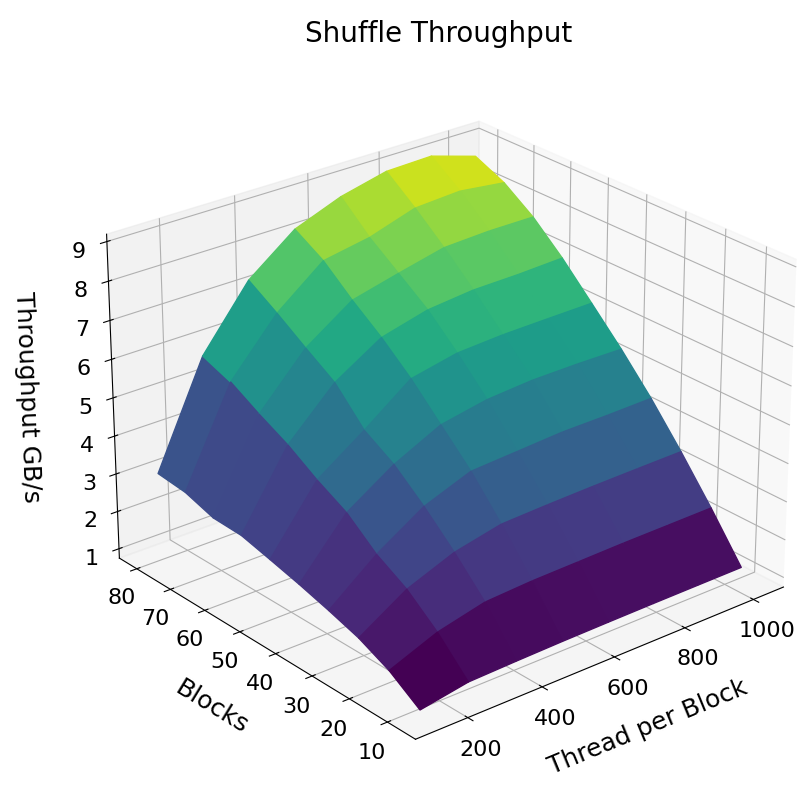
\includegraphics[width=7cm]{images/shuffle_throughput.png}};
%\node<2->[anchor=south east,inner sep=0](image2) at %(200,0){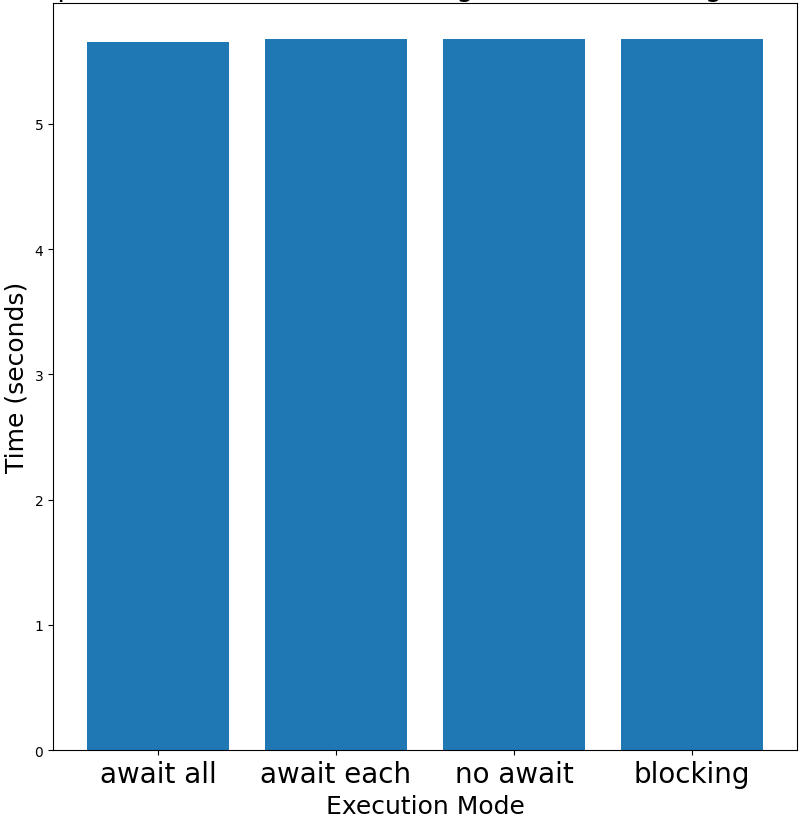
\includegraphics[width=7cm]{images/blocking_nonblocking_barchart.png}};
%\end{tikzpicture}
    \centering
    \begin{tikzpicture}
        \node (shuffle-throughput) {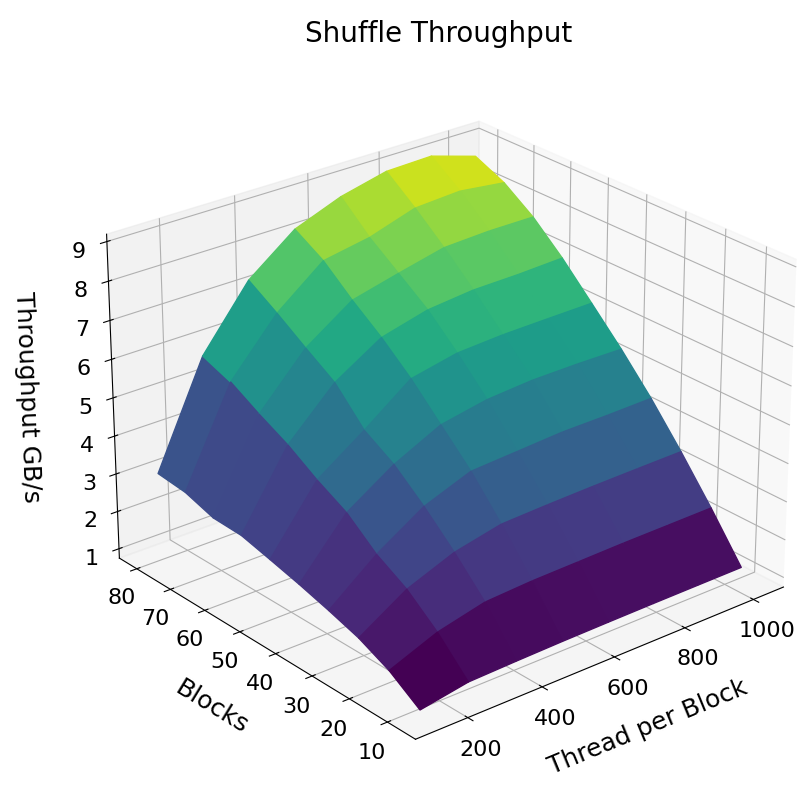
\includegraphics[width=0.4\textwidth]{images/shuffle_throughput.png}};
        \node[right=1em of shuffle-throughput] (scan-speed) {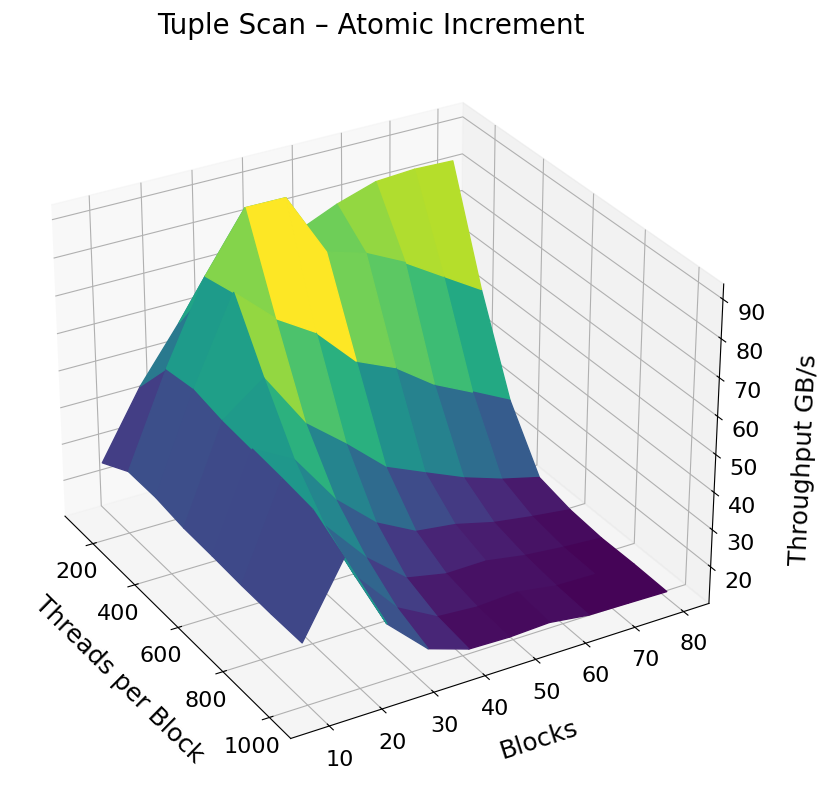
\includegraphics[width=0.4\linewidth]{images/scan_speed_atomic.png}};
        \node<2->[overlay,cloud callout,callout relative pointer={(-1.5cm,-0.8cm)}, line width=0.3mm, draw=black!80,  fill=black!8, aspect=3, align=center, scale=0.8] at ($(shuffle-throughput.center)+(+4.5cm,+3.8cm)$) {May reach full link bandwidth\\with working async interface};
    \end{tikzpicture}
    % \subfloat{}
    % \qquad
    % \subfloat
\end{frame}

\section{Conclusion \& Future work}

\begin{frame}{Contributions}

\begin{itemize}
    \item Explored the performance characteristics of NVSHMEM in a series of benchmarks
    \item Build a GPU-initated shuffle algorithm and benchmark with NVSHMEM
    \item Evaluated multiple algorithmic options for this purpose
\end{itemize}
   
\end{frame}


\begin{frame}{Conclusion}

\begin{itemize}
%    \item TBD: Evaluation of potential for dist. DBs
    \item NVSHMEM performance is non-trivial to understand
    \item GPU-initiated data shuffling might be used to mitigate kernel launch overhead and CPU involvement 
    \item Limitations of our approach:\\
    \begin{itemize}
        \item Requires that all tuples fit into GPU memory
    \end{itemize}
    \item Limitations of NVSHMEM:\\
    \begin{itemize}
        \item HPC style-launch not natural for dist. DBs
        \item Some functionalities are not working as documented w/ newest library version on our hardware
    \end{itemize}
\end{itemize}
% - NVSHMEM has potential for dist. DBs (only valid if luis benchmark shows that kernel launch overhead -does- have a significant impact)
% - Our implementation already incorporates multiple sophisticated techniques but must be further debugged to give an optimal performance
% - Unsolved issue: GPU memory rather limited. If the local partition does not fit into GPU memory, we still need some kind of control flow with the CPU to feed the GPU with data (from CPU mem or from disk). Furthermore, this requires further inter-node communication to notify other nodes when part of the data has been written and can be flushed to disk. This makes it impossible to have completely sync-free sending.
% anything else...?
   
\end{frame}


\section{Credits}

\begin{frame}{Credits}
\framesubtitle{References}

\begin{itemize}
    \item [1] Nvidia, NVSHMEM Documentation, URL: https://docs.nvidia.com/nvshmem/api/, 2023
\end{itemize}
    
\end{frame}

\begin{frame}{Credits}
\framesubtitle{Image Sources}

\begin{itemize}
    \item Title Slide: Nvidia Corp. \textit{https://www.nvidia.com/content/dam/en-zz/Solutions/Data-Center/tesla-v100/data-center-tesla-v100-nvlink-social-image.jpg}
\end{itemize}
    
\end{frame}

\begin{frame}{Backup Slides}
\framesubtitle{Symmetric Memory and NVSHMEM}

\begin{figure}
    \centering
    \begin{tikzpicture}[x=1pt,y=0.9pt,yscale=-0.55,xscale=0.65]
    \begin{tikzpicture}[x=1pt,y=0.9pt,yscale=-0.55,xscale=0.65]
    %Rounded Rect [id:dp5682014849782169] 
    \draw   (100,34.25) .. controls (100,26.52) and (106.27,20.25) .. (114,20.25) -- (156,20.25) .. controls (163.73,20.25) and (170,26.52) .. (170,34.25) -- (170,255.25) .. controls (170,262.98) and (163.73,269.25) .. (156,269.25) -- (114,269.25) .. controls (106.27,269.25) and (100,262.98) .. (100,255.25) -- cycle ;
    %Rounded Rect [id:dp5262477048147362] 
    \draw   (191,34.25) .. controls (191,26.52) and (197.27,20.25) .. (205,20.25) -- (247,20.25) .. controls (254.73,20.25) and (261,26.52) .. (261,34.25) -- (261,255.25) .. controls (261,262.98) and (254.73,269.25) .. (247,269.25) -- (205,269.25) .. controls (197.27,269.25) and (191,262.98) .. (191,255.25) -- cycle ;
    %Rounded Rect [id:dp7573581856079369] 
    \draw   (369,35.25) .. controls (369,27.52) and (375.27,21.25) .. (383,21.25) -- (425,21.25) .. controls (432.73,21.25) and (439,27.52) .. (439,35.25) -- (439,256.25) .. controls (439,263.98) and (432.73,270.25) .. (425,270.25) -- (383,270.25) .. controls (375.27,270.25) and (369,263.98) .. (369,256.25) -- cycle ;
    %Shape: Rectangle [id:dp7570532028079713] 
    \draw  [fill={rgb, 255:red, 208; green, 2; blue, 27 }  ,fill opacity=1 ] (109.42,70.25) -- (161.42,70.25) -- (161.42,109.25) -- (109.42,109.25) -- cycle ;
    %Shape: Rectangle [id:dp19421520470566733] 
    \draw  [fill={rgb, 255:red, 208; green, 2; blue, 27 }  ,fill opacity=1 ] (199.42,71.25) -- (251.42,71.25) -- (251.42,110.25) -- (199.42,110.25) -- cycle ;
    %Shape: Rectangle [id:dp32300543498141965] 
    \draw  [fill={rgb, 255:red, 208; green, 2; blue, 27 }  ,fill opacity=1 ] (379.42,70.25) -- (431.42,70.25) -- (431.42,109.25) -- (379.42,109.25) -- cycle ;
    %Rounded Rect [id:dp6580910781722736] 
    \draw  [fill={rgb, 255:red, 126; green, 211; blue, 33 }  ,fill opacity=1 ] (111.42,141.05) .. controls (111.42,135.64) and (115.8,131.25) .. (121.22,131.25) -- (150.62,131.25) .. controls (156.03,131.25) and (160.42,135.64) .. (160.42,141.05) -- (160.42,190.45) .. controls (160.42,195.86) and (156.03,200.25) .. (150.62,200.25) -- (121.22,200.25) .. controls (115.8,200.25) and (111.42,195.86) .. (111.42,190.45) -- cycle ;
    %Rounded Rect [id:dp26363692092381197] 
    \draw  [fill={rgb, 255:red, 126; green, 211; blue, 33 }  ,fill opacity=1 ] (201.42,141.05) .. controls (201.42,135.64) and (205.8,131.25) .. (211.22,131.25) -- (240.62,131.25) .. controls (246.03,131.25) and (250.42,135.64) .. (250.42,141.05) -- (250.42,190.45) .. controls (250.42,195.86) and (246.03,200.25) .. (240.62,200.25) -- (211.22,200.25) .. controls (205.8,200.25) and (201.42,195.86) .. (201.42,190.45) -- cycle ;
    %Rounded Rect [id:dp18887280028716125] 
    \draw  [fill={rgb, 255:red, 126; green, 211; blue, 33 }  ,fill opacity=1 ] (380.42,140.05) .. controls (380.42,134.64) and (384.8,130.25) .. (390.22,130.25) -- (419.62,130.25) .. controls (425.03,130.25) and (429.42,134.64) .. (429.42,140.05) -- (429.42,189.45) .. controls (429.42,194.86) and (425.03,199.25) .. (419.62,199.25) -- (390.22,199.25) .. controls (384.8,199.25) and (380.42,194.86) .. (380.42,189.45) -- cycle ;
    %Rounded Rect [id:dp5265848887584798] 
    \draw  [color={rgb, 255:red, 0; green, 0; blue, 0 }  ,draw opacity=1 ][dash pattern={on 0.84pt off 2.51pt}] (41.42,64.65) .. controls (41.42,34.05) and (66.22,9.25) .. (96.82,9.25) -- (445.02,9.25) .. controls (475.61,9.25) and (500.42,34.05) .. (500.42,64.65) -- (500.42,230.85) .. controls (500.42,261.45) and (475.61,286.25) .. (445.02,286.25) -- (96.82,286.25) .. controls (66.22,286.25) and (41.42,261.45) .. (41.42,230.85) -- cycle ;
    %Shape: Rectangle [id:dp9039242900086101] 
    \draw  [color={rgb, 255:red, 245; green, 166; blue, 35 }  ,draw opacity=1 ][dash pattern={on 5.63pt off 4.5pt}][line width=1.5]  (106,121) -- (433.42,121) -- (433.42,210.25) -- (106,210.25) -- cycle ;
    
    % Text Node
    \draw (135.26,34.5) node   [align=left] {PE 0};
    % Text Node
    \draw (225.26,34.5) node   [align=left] {PE 1};
    % Text Node
    \draw (405.26,34.5) node   [align=left] {PE 2};
    % Text Node
    \draw (510,272) node [anchor=north west][inner sep=0.8pt]  [rotate=-270] [align=left] {NVSHMEM\_TEAM\_WORLD};
    % Text Node
    \draw (280,145) node [anchor=north west][inner sep=0.75pt]   [align=center] {Symmetric \\ Memory};
\end{tikzpicture}

    \end{tikzpicture}
    \caption{NVSHMEM symmetric memory model (Adapted from [1])}
    \label{fig:my_label}
\end{figure}

\end{frame}

%\begin{frame}{Backup Slides}
%\framesubtitle{Tuple Scan Speed Atomic Insert}
%\vspace{-4.0mm}
%\begin{center}
%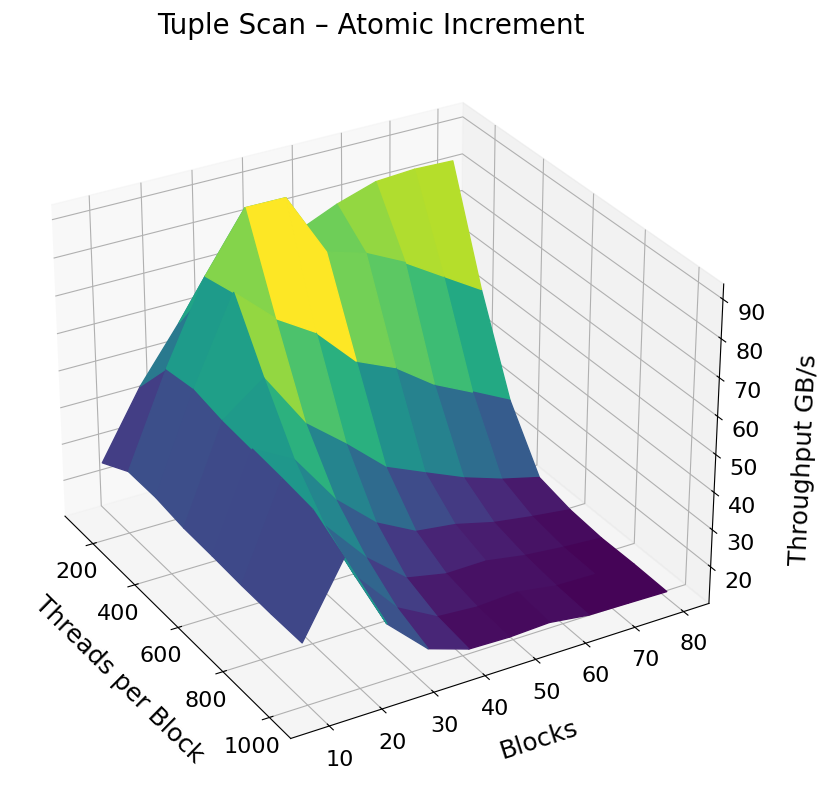
\includegraphics[width=0.45\linewidth]{images/scan_speed_atomic.png}
%\end{center}
%\end{frame}


\begin{frame}{Backup Slides}
\framesubtitle{Throughput Difference Atomic Add - Sync-free}
\vspace{-4.0mm}
\begin{center}
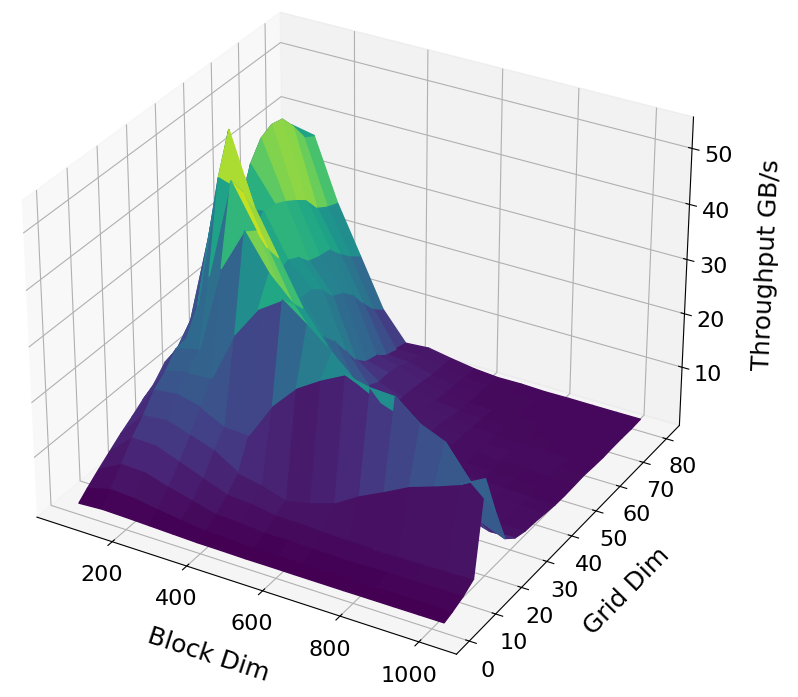
\includegraphics[width=0.45\linewidth]{images/scan_speed_diff.png}
\end{center}
\end{frame}

\begin{frame}{Backup Slides}
\framesubtitle{Comparison of NVSHMEM execution modes}
\vspace{-2.0mm}
\begin{center}
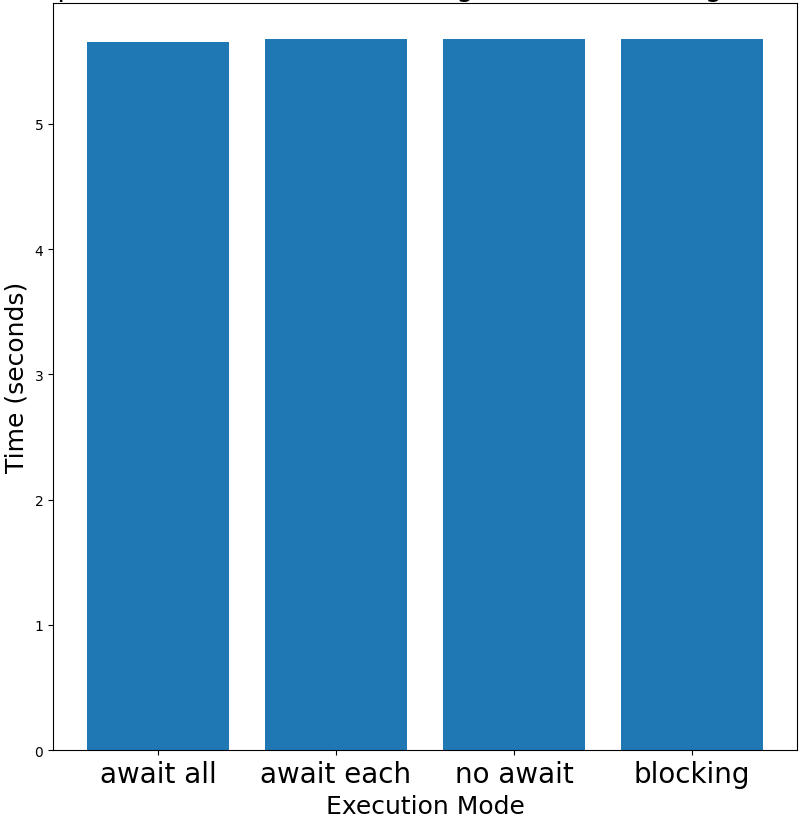
\includegraphics[width=0.38\linewidth]{images/blocking_nonblocking_barchart.png}
\end{center}
\end{frame}


%\begin{frame}{Backup Slides}
%\framesubtitle{NVSHMEM communication and synchronization primitives}


%TODO!
    
%\end{frame}



% for reference purposes
%\begin{frame}{Hinweis zur Ausrichtung (insbesondere columns)}
	%Die Standardausrichtung wurde gegenüber den Beamer-Voreinstellungen von \code{c} zu \code{t} geändert. Dies bedeutet, dass Inhalt auf der Folie oben ausgerichtet wird. Dies entspricht den Vorgaben, hat allerdings den Nachteil, dass die \code{columns}-Umgebung in diesem Fall bei der Positionierung von Bildern ungewohnte Ergebnisse erzeugt.

	%Die Ausrichtung kann in diesem Fall entweder global mit der Option \code{c} wieder zum Standard geändert werden, oder aber das \code{c} wird direkt an die \code{columns}-Umgebung übergeben. Zum Beispiel:
%\begin{columns}[onlytextwidth,c]%ohne das c ist die Ausrichtung verschoben
	%\column{.8\linewidth}
	%\begin{itemize}
	%	\item eins
	%	\item zwei
	%\end{itemize}
	%\column{.2\linewidth}
	%\includegraphics[width=\linewidth]{example-image}
%\end{columns}
%\end{frame}

\end{document}

% 1:
% - Welcome to our presentation about Benchmarking NVSHMEM for distributed data shuffling
% - My name is ..., this is ..., other authors are ..., supervisors are ...
% 
% 2:
% - Let's start with a motivation of our topic: 
% - Common scenario: CPU launches a GPU kernel for the acceleration of computation
% - In distributed systems: GPU kernel finishes and CPU sends data to remote node
% - Continue for next batch of the data with a new kernel
% - Problem: CPU usage higher and kernel launch overhead
%     - -> rather use speech bubbles for the issue and then right figure for the solution. Remove slide 3 then
% 
% 3:  
% - For example, here we have plotted the execution time of calculations on the GPU using a single kernel (red) and multiple kernels (blue) for the same problem.
% - The larger the problem gets, i.e. the more kernels we have to launch for the subproblems in the blue line, the more we suffer from the overhead of launching kernels.
% - This is one of the things we can improve using GPU initiated communication, since the control does not have to return to the CPU for sending
% 
% 4:
% - Let's look at today's outline
% - We have just looked into a motivation for GPU-initiated network communication.
% - Next we will explain how this can be used for the use case of distributed data shuffling
% - After that, we will show benchmarks results of NVSHMEM communication primitives and based on that construct our own shuffle implementation using NVSHMEM for GPU-initiated communication
% - Then, we evaluate our implementation with a benchmark and conclude the findings of our project work
% 
% 5:
% - Join is one of the most common and most expensive operations in distributed database management systems
% - So, it makes sense to optimize the join
% - If the tuples are not distributed to the join key, they have to be redistributed, so the key matching can be performed locally. This is called shuffling
% - Using GPUs for shuffling can make the scanning a lot faster due to massive parallelization. But we also have to optimize the sending for this network-intensive operation
% 
% 6: (comic)
% - When designing a shuffle with GPU-initiated RDMA, there are several questions coming up:
%     - coordination of remote memory?
%     - parallel sending?
%     - frequency of sending?
% 
% 7:
% - To begin with, to understand the differenc between CPU- and GPU-initiated communication better, we have plotted the BW of one CPU thread and one GPU thread when sending data packets of different sizes using GPUDirect RDMA
% - Since CPUs have a higher clock frequency and more specialized instruction set, they can execute the necessary control flow faster
% - Eventually, both methods max out just below the network bandwidth, which is at 12.5 GB/s
% - But the good news is, with GPUs we can also compute more data parallely and we might benefit from parallelized sending
% 
% 8:
% - So let us take a look at how sending with multiple GPU threads parallelizes when using NVSHMEM.
% - We see different message sizes on the x-axis and the throuput on the y-axis.
% - First of all, we see that we need a certain minimum message size in order to get good performance. So NVSHMEM seems to not buffer calls in the background and direct tuple-wise sending is not an option. We need to assemble multiple tuples in a batch for sending.
% - As one can see, it seems like for some reason the performance gets worse if we use more threads in a block
% - But what happens if we increase the number of blocks?
% 
% 9:
% - We now see that the performance of one thread for sending decreases and using more threads per block seems to be better
% - This is one of the strange behaviours that we have seen when using NVSHMEM
% - For our implementation, this means if we use one thread for sending and a large enough send buffer, we should get quite good and predictable behaviour
% 
% 10:
% - Let's look at some important highlights of our implementation, which is inspired by the benchmark results that we have just seen
% - Since we use one sided RDMA, we need to know what positions to write to on the destionation
% - For this we first compute local histograms of our local key column to know how many tuples each node has for each destionation
% - Then we exchange the histograms using the fcollect NVSHMEM primitive, which we by the way had to reimplement because it did not work in release mode
% - Finally, we compute the offsets the prefix sum for the nodes locally
% 
% 11:
% - Now that we know the remote addresses for writing, we want to rescan the data and send it.
% - Based on our findings in the benchmarks, we use send buffers of sufficient size.
% - For synchronization reasons, one send buffer per destination, per thread block
% - When inserting into the buffers, we increment an atomic pointer to coordinate the GPU threads
% - Once the buffers are full, we initiate the sending with an NVSHMEM non-blocking call and use one thread for that
% - We thenswap buffers and continue computing right away to balance compute and networking
% 
% 12:
% - We have then benchmarked our implementation of the shuffle
% - We see that when using a larger number of threads, the performance grows, which makes sense because we scan the data at a higher rate
% - The peak throughput we get is around 9 GB/s, (remember BW is at 12.5, also metadata not counted here)
% - Since our goal was to get as close to BW as possible, we investigated any bottlenecks of our implementation.
% - We saw that the scan alone without sending worked fine and was much faster than 12.5 GB/s
% - We then found out that the NVSHMEM non-blocking interface did not work as documented in our setup.
% - For this reason, our implementation of double buffering could not work correctly
% - If the issue is fixed in a future library version, our implementation might get very close to 12 GB/s
% 
% 13:
% - To sum up the contributions:
% - ...
% 
% 14:
% - Let us finish off with a conclusion of our project
% - We have found out that NVSHMEMs performance is nontrivial in many ways and that this makes it hard to use it in a performant way
% - Our implementation shows that NVSHMEM is usuable for data shuffling and might be used to reduce kernel launch overhead and CPU involvement
% - our approach need all tuples in GPU mem at same time
% - nvshmem is not nice for dist DBMSs in terms of launching, no runtime resource adjustment possible
% - Some library functionalities like fcollect, signals and the non-blocking interface did not work as expected on our hardware
% 
% 